% Template for PLoS
% Version 3.6 Aug 2022
%
% % % % % % % % % % % % % % % % % % % % % %
%
% -- IMPORTANT NOTE
%
% This template contains comments intended 
% to minimize problems and delays during our production 
% process. Please follow the template instructions
% whenever possible.
%
% % % % % % % % % % % % % % % % % % % % % % % 
%
% Once your paper is accepted for publication, 
% PLEASE REMOVE ALL TRACKED CHANGES in this file 
% and leave only the final text of your manuscript. 
% PLOS recommends the use of latexdiff to track changes during review, as this will help to maintain a clean tex file.
% Visit https://www.ctan.org/pkg/latexdiff?lang=en for info or contact us at latex@plos.org.
%
%
% There are no restrictions on package use within the LaTeX files except that no packages listed in the template may be deleted.
%
% Please do not include colors or graphics in the text.
%
% The manuscript LaTeX source should be contained within a single file (do not use \input, \externaldocument, or similar commands).
%
% % % % % % % % % % % % % % % % % % % % % % %
%
% -- FIGURES AND TABLES
%
% Please include tables/figure captions directly after the paragraph where they are first cited in the text.
%
% DO NOT INCLUDE GRAPHICS IN YOUR MANUSCRIPT
% - Figures should be uploaded separately from your manuscript file. 
% - Figures generated using LaTeX should be extracted and removed from the PDF before submission. 
% - Figures containing multiple panels/subfigures must be combined into one image file before submission.
% For figure citations, please use "Fig" instead of "Figure".
% See http://journals.plos.org/plosone/s/figures for PLOS figure guidelines.
%
% Tables should be cell-based and may not contain:
% - spacing/line breaks within cells to alter layout or alignment
% - do not nest tabular environments (no tabular environments within tabular environments)
% - no graphics or colored text (cell background color/shading OK)
% See http://journals.plos.org/plosone/s/tables for table guidelines.
%
% For tables that exceed the width of the text column, use the adjustwidth environment as illustrated in the example table in text below.
%
% % % % % % % % % % % % % % % % % % % % % % % %
%
% -- EQUATIONS, MATH SYMBOLS, SUBSCRIPTS, AND SUPERSCRIPTS
%
% IMPORTANT
% Below are a few tips to help format your equations and other special characters according to our specifications. For more tips to help reduce the possibility of formatting errors during conversion, please see our LaTeX guidelines at http://journals.plos.org/plosone/s/latex
%
% For inline equations, please be sure to include all portions of an equation in the math environment.  For example, x$^2$ is incorrect; this should be formatted as $x^2$ (or $\mathrm{x}^2$ if the romanized font is desired).
%
% Do not include text that is not math in the math environment. For example, CO2 should be written as CO\textsubscript{2} instead of CO$_2$.
%
% Please add line breaks to long display equations when possible in order to fit size of the column. 
%
% For inline equations, please do not include punctuation (commas, etc) within the math environment unless this is part of the equation.
%
% When adding superscript or subscripts outside of brackets/braces, please group using {}.  For example, change "[U(D,E,\gamma)]^2" to "{[U(D,E,\gamma)]}^2". 
%
% Do not use \cal for caligraphic font.  Instead, use \mathcal{}
%
% % % % % % % % % % % % % % % % % % % % % % % % 
%
% Please contact latex@plos.org with any questions.
%
% % % % % % % % % % % % % % % % % % % % % % % %

\documentclass[10pt,letterpaper]{article}
\usepackage[top=0.85in,left=2.75in,footskip=0.75in]{geometry}

% amsmath and amssymb packages, useful for mathematical formulas and symbols
\usepackage{amsmath,amssymb}

% Use adjustwidth environment to exceed column width (see example table in text)
\usepackage{changepage}

% textcomp package and marvosym package for additional characters
\usepackage{textcomp,marvosym}

% cite package, to clean up citations in the main text. Do not remove.
\usepackage{cite}

% Use nameref to cite supporting information files (see Supporting Information section for more info)
\usepackage{nameref,hyperref}

% line numbers
\usepackage[right]{lineno}

% ligatures disabled
\usepackage[nopatch=eqnum]{microtype}
\DisableLigatures[f]{encoding = *, family = * }

% color can be used to apply background shading to table cells only
\usepackage[table]{xcolor}
\hypersetup{
    colorlinks,
    linkcolor={red!50!black},
    citecolor={blue!50!black},
    urlcolor={blue!80!black}
}

% array package and thick rules for tables
\usepackage{array}

% create "+" rule type for thick vertical lines
\newcolumntype{+}{!{\vrule width 2pt}}

% create \thickcline for thick horizontal lines of variable length
\newlength\savedwidth
\newcommand\thickcline[1]{%
  \noalign{\global\savedwidth\arrayrulewidth\global\arrayrulewidth 2pt}%
  \cline{#1}%
  \noalign{\vskip\arrayrulewidth}%
  \noalign{\global\arrayrulewidth\savedwidth}%
}

% \thickhline command for thick horizontal lines that span the table
\newcommand\thickhline{\noalign{\global\savedwidth\arrayrulewidth\global\arrayrulewidth 2pt}%
\hline
\noalign{\global\arrayrulewidth\savedwidth}}


% Remove comment for double spacing
%\usepackage{setspace} 
%\doublespacing

% Text layout
\raggedright
\setlength{\parindent}{0.5cm}
\textwidth 5.25in 
\textheight 8.75in

% Bold the 'Figure #' in the caption and separate it from the title/caption with a period
% Captions will be left justified
\usepackage[aboveskip=1pt,labelfont=bf,labelsep=period,justification=raggedright,singlelinecheck=off]{caption}
\renewcommand{\figurename}{Fig}


% Use the PLoS provided BiBTeX style
\bibliographystyle{plos2015}

% Remove brackets from numbering in List of References
\makeatletter
\renewcommand{\@biblabel}[1]{\quad#1.}
\makeatother



% Header and Footer with logo
\usepackage{lastpage,fancyhdr,graphicx}
\usepackage{epstopdf}
%\pagestyle{myheadings}
\pagestyle{fancy}
\fancyhf{}
%\setlength{\headheight}{27.023pt}
%\lhead{\includegraphics[width=2.0in]{PLOS-submission.eps}}
\rfoot{\thepage/\pageref{LastPage}}
\renewcommand{\headrulewidth}{0pt}
\renewcommand{\footrule}{\hrule height 2pt \vspace{2mm}}
\fancyheadoffset[L]{2.25in}
\fancyfootoffset[L]{2.25in}
\lfoot{\today}

%% Include all macros below

\newcommand{\lorem}{{\bf LOREM}}
\newcommand{\ipsum}{{\bf IPSUM}}

%% END MACROS SECTION


\begin{document}
\vspace*{0.2in}

% Title must be 250 characters or less.
\begin{flushleft}
{\Large
\textbf\newline{Recording provenance of workflow runs with RO-Crate} % Please use "sentence case" for title and headings (capitalize only the first word in a title (or heading), the first word in a subtitle (or subheading), and any proper nouns).
}
\newline
% Insert author names, affiliations and corresponding author email (do not include titles, positions, or degrees).
\\

Simone Leo\textsuperscript{1*},
Michael R. Crusoe\textsuperscript{2,3,4},
Laura Rodríguez-Navas\textsuperscript{5}, 
Raül Sirvent\textsuperscript{5}, 
Alexander Kanitz\textsuperscript{6,7}, 
Paul De Geest\textsuperscript{8}, 
Rudolf Wittner\textsuperscript{9,10,11}, 
Luca Pireddu\textsuperscript{1}, 
Daniel Garijo\textsuperscript{12}, 
José M. Fernández\textsuperscript{5}, 
Iacopo Colonnelli\textsuperscript{13}, 
Matej Gallo\textsuperscript{9}, 
Tazro Ohta\textsuperscript{14,15}, 
Hirotaka Suetake\textsuperscript{16}, 
Salvador Capella-Gutierrez\textsuperscript{5}, 
Renske de Wit\textsuperscript{2}, 
Bruno de Paula Kinoshita\textsuperscript{5}, 
Stian Soiland-Reyes\textsuperscript{17,18}
\\
\bigskip
\textbf{1} Center for Advanced Studies, Research, and Development in Sardinia (CRS4), Pula, Sardinia, Italy
\\
\textbf{2} Vrije Universiteit Amsterdam, Amsterdam, The Netherlands
\\
\textbf{3} DTL Projects, The Netherlands
\\
\textbf{4} Forschungszentrum Jülich, Germany
\\
\textbf{5} Barcelona Supercomputing Center, Barcelona, Spain
\\
\textbf{6} Biozentrum, University of Basel, Basel, Switzerland
\\
\textbf{7} Swiss Institute of Bioinformatics, Lausanne, Switzerland
\\
\textbf{8} VIB-UGent Center for Plant Systems Biology, Gent, Belgium
\\
\textbf{9} Faculty of Informatics, Masaryk University, Brno, Czech Republic
\\
\textbf{10} Institute of Computer Science, Masaryk University, Brno, Czech Republic
\\
\textbf{11} BBMRI-ERIC, Graz, Austria
\\
\textbf{12} Ontology Engineering Group, Universidad Politécnica de Madrid, Madrid, Spain
\\
\textbf{13} Computer Science Dept., Università degli Studi di Torino, Torino, Italy
\\
\textbf{14} Database Center for Life Science, Joint Support-Center for Data Science Research, Research Organization of Information and Systems, Shizuoka, Japan
\\
\textbf{15} Institute for Advanced Academic Research, Chiba University, Chiba, Japan
\\
\textbf{16} Department of Creative Informatics, Graduate School of Information Science and Technology, The University of Tokyo, Tokyo, Japan
\\
\textbf{17} Department of Computer Science, The University of Manchester, Manchester, United Kingdom
\\
\textbf{18} Informatics Institute, University of Amsterdam, Amsterdam, The Netherlands
\\
\bigskip

% Insert additional author notes using the symbols described below. Insert symbol callouts after author names as necessary.
% 
% Remove or comment out the author notes below if they aren't used.
%
% Primary Equal Contribution Note
%\Yinyang These authors contributed equally to this work.

% Additional Equal Contribution Note
% Also use this double-dagger symbol for special authorship notes, such as senior authorship.
%\ddag These authors also contributed equally to this work.

% Current address notes
%\textcurrency Current Address: Dept/Program/Center, Institution Name, City, State, Country % change symbol to "\textcurrency a" if more than one current address note
% \textcurrency b Insert second current address 
% \textcurrency c Insert third current address

% Deceased author note
%\dag Deceased

% Group/Consortium Author Note
%\textpilcrow Membership list can be found in the Acknowledgments section.

% Use the asterisk to denote corresponding authorship and provide email address in note below.
* simone.leo@crs4.it

\end{flushleft}
% Please keep the abstract below 300 words
\section*{Abstract}
Recording the provenance of scientific computation results is
key to the support of traceability, reproducibility and quality
assessment of data products. Several data models have been explored to
address this need, providing representations of workflow plans and their
executions as well as means of packaging the resulting information for
archiving and sharing. However, existing approaches tend to lack fine-grained interoperability and adoption from workflow management systems. In this work we present
Workflow Run RO-Crate, an extension of RO-Crate (Research Object Crate)
to capture the provenance of the execution of computational workflows at
different levels of granularity an bundle together all their associated products (inputs, outputs, code etc.). We describe the model, as well as its
implementations in six workflow systems, and show its applicability to
machine learning for digital pathology use cases. The model is supported
by a diverse, open community that runs regular meetings, discussing
development, maintenance and adoption  aspects. The format is already implemented by
several workflow managers, including Galaxy, allowing interoperable
comparisons between runs from heterogeneous systems.


% Disable for preprint
\linenumbers



\emph{The below is a snapshot as of 2023-09-07 from
\url{https://docs.google.com/document/d/1rq22Vu_lmmRLkmnZivsKVdRidq4aoePs-l20gHFYpu0/edit}}.

\section{Introduction}\label{introduction}

A crucial part of scientific research is recording the provenance of its outputs.
The W3C PROV standard defines provenance as ``a record that describes the people, institutions, entities, and activities involved in producing, influencing, or delivering a piece of data or a thing''
\cite{Moreau 2013}.
Provenance is instrumental to activities such as traceability, reproducibility, accountability, and quality assessment
\cite{Herschel 2017}.
The constantly growing size and complexity of scientific datasets and the analysis that is required to extract useful information from them has made science increasingly dependent on advanced automated processing techniques in order to get from experimental data to final results~\cite{Himanen 2019, Gauthier 2019, Huntingford 2019}.
Consequently, a large part of the provenance information for scientific outputs consists of descriptions of complex computer-aided data processing steps.

In order to homogenise the collection and interchange of provenance records, the W3C consortium proposed the PROV-O standard~\cite{Lebo 2013}, a machine-readable OWL \cite{W3C OWL Working Group 2012} representation of PROV for provenance in the Web.
PROV-O has been widely extended for workflows (D-PROV \cite{Missier 2013}, ProvONE \cite{Cuevas-Vicenttín 2016}, OPMW \cite{Garijo 2011}, P-PLAN \cite{Garijo 2012}), where provenance information is collected in two main forms: prospective and retrospective~\cite{Freire 2008}. \emph{Prospective provenance}, i.e.~the execution plan, is essentially the workflow itself: it includes a machine-readable specification with the processing steps to perform and the data and software dependencies to carry out each computation.
\emph{Retrospective provenance} refers to what actually happened during an execution, i.e.~what were the values of the input parameters, which outputs were produced, which tools were executed, how much time did the execution take, whether the execution was successful or not, etc.
Retrospective provenance can also be represented at different levels of abstraction depending on available computing resources, e.g.~by the workflow execution becoming a single activity which produces results, by specifying the individual execution of each workflow step, or by going a step further and indicating how each step is further divided into sub-processes when a workflow is deployed in a cluster.

Different workflow systems have adopted and extended PROV (and its PROV-O representation) to the workflow domain (Pegasus \cite{Deelman 2005}, VsTrails \cite{Scheidegger 2008}), in order to ease the burden of provenance collection from tool developers to workflow management systems (WMSs) \cite{Atkinson 2017}.

D-PROV, PROV-ONE, OPMW-PROV, P-Plan propose representations of workflow plans and their respective executions, taking into account the features of the workflow systems implementing them (e.g., hierarchical representations, sub-processes, etc.).
Other data models like \emph{wfprov} and \emph{wfdesc}
\cite{Belhajjame 2015} go a step further by considering not only the link between plans and executions, but how to package everything as a Research Object~\cite{Bechhofer 2013} in order to ease portability while keeping the context of a digital experiment.
However, while these data models address some workflow provenance representation issues, they have two main limitations: first, the extensions are not interoperable at lower levels of granularity, due to different assumptions in workflow representation.
Second, they lack support from workflow management systems (WMS).

These problems have been partially addressed by CWLProv~\cite{Khan 2019}, which represents the workflow enactment as ROs serialised according to the BDBag approach~\cite{Chard 2016}.
The resulting format is a folder containing several data and metadata files~\cite{Soiland-Reyes 2018}.
CWLProv also extends PROV with a representation of executed processes (activities), their inputs and outputs (entities) and their executors (agents), together with their Common Workflow Language specification
\cite{Crusoe 2022}, a standard workflow specification adopted by at least a dozen different workflow systems (\url{https://www.commonwl.org/implementations/}). Although CWLProv includes a prospective provenance as a \emph{plan}
within PROV (based on the \emph{wfdesc} model), in practice its implementation does not include tool definitions or file formats, as proposed by the wfdesc extension Roterms (\url{https://wf4ever.github.io/ro/2016-01-28/roterms}).
In order for CWLProv consumers to reconstruct the full prospective provenance for understanding the workflow, they would also need to inspect the separate workflow definition in the WMS's native language.
Additionally, the CWLProv RO may include several other BagIt metadata files and PROV serialisations conforming to different formats, complicating its generation and consumption.
CWLProv proposed multiple levels of provenance \cite[figure 2]{Khan 2019}, from Level 0 (capturing workflow definition) to Level 3 (domain-specific annotations). 
In practice, the CWL reference implementation \emph{cwltool} \cite{Amstutz 2023} records provenance details of all task executions together with the intermediate data and any nested workflows (CWLProv level 2), a granularity level that requires substantial support from the WMS
\cite{Soiland-Reyes 2022a}.
This approach, while appropriate for workflow languages where the execution plan, including its distribution among the various tasks, is well known in advance (such as CWL), can be at odds with other systems where the execution is more dynamic, depending on the verification of specific runtime conditions, such as the size and distribution of the data (e.g., COMPSs~\cite{Lordan 2014}).
This makes the implementation of CWLProv challenging, as shown by the fact that at the time of writing the format is supported only by cwltool.
Finally, being based on the PROV model, CWLProv is highly focused on the interaction between agents, processes and related entities, while support for contextual metadata (such as workflow authors, licence or creation date) in the Research Object is limited (\url{https://w3id.org/bundle/context}) and stored in a separate manifest file.

RO-Crate~\cite{Soiland-Reyes 2022a} is a recent approach to packaging research data together with their metadatal; it extends Schema.org~\cite{Guha 2015}, a popular vocabulary for describing resources on the Web.
In its simplest form, an RO-Crate is a directory structure that contains a single JSON-LD metadata file at the top level.
The metadata file describes all entities stored in the RO-Crate along with as their relationships; it is both machine-readable and human-readable.
The format is general enough to be able to describe any dataset, but can also be made as specific as needed through the use of extensions called
\emph{profiles}.
At the same time, the broad set of types and properties from Schema.org, complemented by a few additional terms from other vocabularies, make the RO-Crate model capable of expressing a wide range of contextual information that complements and enriches the core information specified by the profile.
This might include, for instance, the workflow authors and their affiliations, associated publications, licensing information, related software, etc.

In this work, we present Workflow Run RO-Crate (WRROC), an extension of RO-Crate for representing computational workflow provenance.
Our main contributions are the following:

\begin{itemize}
\item   A collection of RO-Crate profiles to represent both the prospective and the retrospective provenance of a computational   workflow run in a way that is machine-actionable,  independent of the specific  workflow language or   execution system, and including support for rerunnability.
\item   Implementations of the model in XX workflow systems.
\item   A governance and sustainability environment to discuss extensions,  issues and new implementations for the proposed   profiles, possible thanks to the WRROC community.
\end{itemize}

To foster usability, the profiles are characterised by different levels of detail, and set of mandatory metadata items is kept to a minimum in order to ease the implementation.
This flexible approach increases the model's adaptability to the diverse landscape of WMSs used in practice.
The base profile, in particular, is applicable to any kind of computational process, not necessarily described in a formal workflow language.
In this work we describe several implementations and demonstrate the application to multiple use cases.

The rest of this paper is organised as follows: we first describe the Workflow Run RO-Crate profiles; we then illustrate implementations and usage examples; this is followed by a discussion and plans for future work.


%% 
\section{The Workflow Run RO-Crate profiles}\label{the-workflow-run-ro-crate-profiles}

The Workflow Run RO-Crate profiles are a set of RO-Crate profiles, 
extensions of the base RO-Crate specification that describes how to represent the entities and relationships that appear in a specific domain or use case.
An RO-Crate conforming to a profile is not just machine-readable, but also machine-actionable as a digital object whose type is represented by the profile itself~\cite{Soiland-Reyes 2022c}.

The Workflow Run RO-Crate profiles are the main outcome of the Workflow Run RO-Crate Community (\url{https://www.researchobject.org/workflow-run-crate}), an open working group that includes workflow users and developers, WMS users and developers, and researchers and software engineers interested in workflow execution provenance and FAIR approaches for data and software.
In order to develop the Workflow-Run RO-Crate profile, one of the first community efforts was to compile a list of requirements in the form of competency questions (\url{https://www.researchobject.org/workflow-run-crate/requirements}) to be addressed by the model.
Each requirement was backed up by a rationale and linked to a GitHub issue to drive the discussion forward. When a requirement was addressed, related changes were integrated into the profiles and the relevant issue was closed. Many of the original issues are now closed, and the profiles have had two official releases.


As requirements were being defined, it became apparent that one single profile would not have been sufficient to cater to all possible usage scenarios.
In particular, while some use cases required a detailed description of all computations orchestrated by the workflow, others were only concerned with a ``black box'' representation of the workflow and its execution as a whole.
Additionally, some computations involve a data flow across multiple applications; that are executed without the aid of a WMS and thus are not formally described in a standard workflow language.
These observations led to the development of three profiles: 
(1) Process Run Crate (\url{https://w3id.org/ro/wfrun/process/0.1})
\cite{Workflow Run RO-Crate working group 2023a} to describe the execution of one or more tools that contribute to a computation;
(2) Workflow Run Crate (\url{https://w3id.org/ro/wfrun/workflow/0.1})
\cite{Workflow Run RO-Crate working group 2023b} to describe a computation orchestrated by a predefined workflow; 
(3) Provenance Run Crate (\url{https://w3id.org/ro/wfrun/provenance/0.1})
\cite{Workflow Run RO-Crate working group 2023c} to describe a workflow computation including the internal details of individual step executions.

In the rest of this section we describe each of the above profiles in detail.
We use italics to denote the types and properties used to describe entities and their relationships: these are defined in the RO-Crate JSON-LD context (\url{https://www.researchobject.org/ro-crate/1.1/context.jsonld}), which extends Schema.org with terms from the Bioschemas \cite{Gray 2017} ComputationalWorkflow profile (\url{https://bioschemas.org/profiles/ComputationalWorkflow/1.0-RELEASE}) and other vocabularies. More specifically, we use the \emph{ComputationalWorkflow} and \emph{FormalParameter} types as well as the \emph{input} and \emph{output} properties. We also developed a context extension through a dedicated "workflow-run" namespace in ro-terms (https://w3id.org/ro/terms/workflow-run\#) to represent concepts that are not captured by terms in the RO-Crate context.

\subsection{Process Run Crate}\label{process-run-crate}

The Process Run Crate profile contains guidelines on describing the execution of one or more software applications that contribute to the same overall computation, but are not necessarily coordinated by a top-level workflow or script.
For instance, they could be executed manually by a human agent, one after the other as intermediate datasets become available.

Being the basis for all profiles in the WRROC collection, Process Run Crate specifies how to describe the fundamental entities involved in a computational run: a software application (represented by
\emph{SoftwareApplication}, \emph{SoftwareSourceCode} or
\emph{ComputationalWorkflow} entities) and its execution (represented by a \emph{CreateAction} entity), with the latter linking to the former via the \emph{instrument} property.
Other important properties of the
\emph{CreateAction} entity are \emph{object}, which links to the action's inputs, and \emph{result}, which links to its outputs.
The time the execution started and ended can be provided, respectively, via the
\emph{startTime} and \emph{endTime} properties.
The \emph{Person} or
\emph{Organization} entity that performed the action is referred to via the \emph{agent} property.
Fig~\ref{fig:process_crate_er} shows the entities used in Process Run Crate together with their relationships.

\begin{figure}[!h]
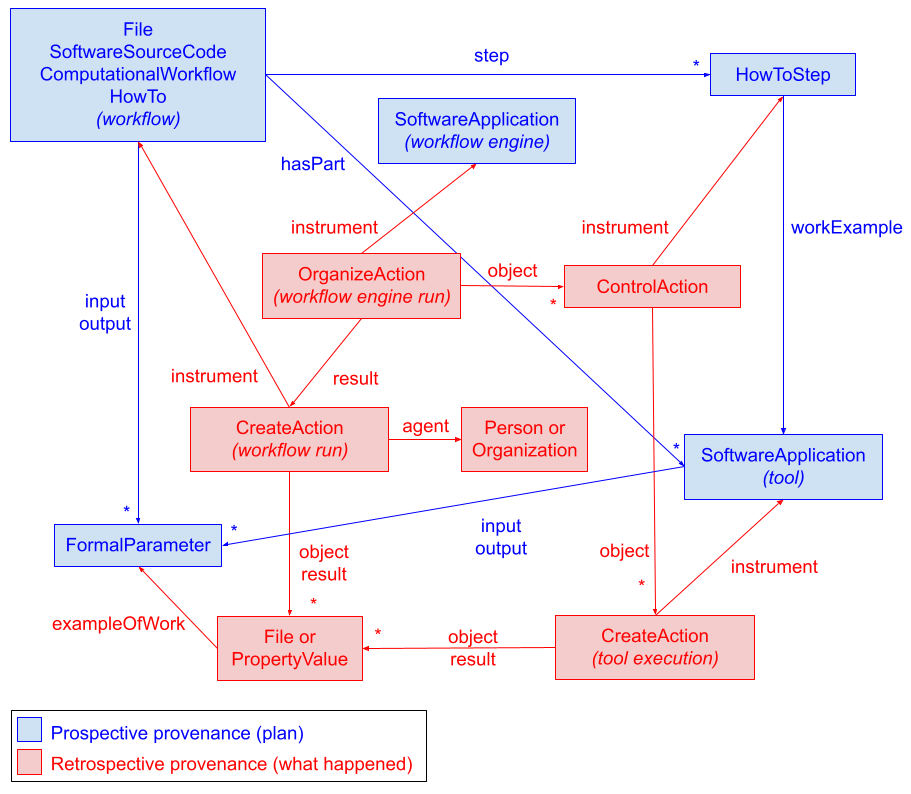
\includegraphics[width=\textwidth]{image1.png}
\caption{{\bf Entity-Relationship diagram for Process Run Crate.}
The central entity is the \emph{CreateAction}, which represents the execution of an application.
It relates with the application itself via \emph{instrument}, with the entity that executed it via \emph{agent} and with its inputs and outputs via \emph{object}
and \emph{result}, respectively. 
\emph{File} is an RO-Crate alias for Schema.org's \emph{MediaObject}}
\label{fig:process_crate_er}
\end{figure}

As an example,
suppose a user called John Doe runs the ``head'' UNIX command to extract the first ten lines of an input file called lines.txt, storing the result in another file called selection.txt.
Then, the same user runs the ``sort''
command on selection.txt, storing the sorted output in a file called sorted\_selection.txt.
Fig~\ref{fig:head_sort} contains a diagram of the two actions and their relationships to the other entities involved.
Note how the actions are connected by the fact that the output of ``Run Head'' is also the input of ``Run Sort'': they form an ``implicit workflow'', whose steps have been executed manually rather than by a higher level software tool.

%% gdoc updates until here

\begin{figure}[!h]
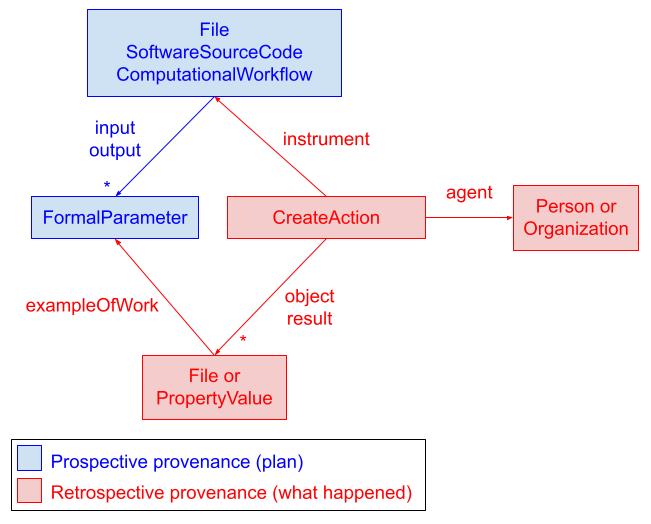
\includegraphics[width=29em]{image2.png}
\caption{{\bf Diagram of a simple workflow} where the head and sort programs were run manually by a user.
The executions of the individual software programs are connected by the fact that the file output by head was used as input for sort, documenting the computational flow in an implicit way.
Such executions can be represented with Process Run Crate.}
\label{fig:head_sort}
\end{figure}


Process Run Crate extends the RO-Crate guidelines on representing software used to create files with additional requirements and conventions.
This arrangement is typical of the RO-Crate approach, where the base specification provides general recommendations to allow for high flexibility, while profiles, being more concerned with the representation of specific domains and machine actionability, provide more detailed and structured definitions.
Nevertheless, in order to be broadly applicable, profiles also need to avoid the specification of too many strict requirements, trying to strike a good trade-off between flexibility and actionability.
One of the implications of this approach is that consumers need to code defensively, avoiding unwarranted assumptions – e.g., by verifying that a value exists for an optional property before trying to retrieve it and use it.

While containing its degree of complexity, the Process Run Crate profile already addresses many of the requirements collected through the community competency questions. 
For instance, the profile can be used to work with “composite” datasets consisting of multiple files and directories to be treated as a single unit – as opposed to more conventional input or output parameters consisting of a single file;
this occurs, for instance, with some digital image formats where a single image can be stored across multiple data and metadata files.
The profile specifies that such datasets should be represented by a
\emph{Collection} entity linking to individual files and directories via the \emph{hasPart} property, and referencing the main part (if any) via the \emph{mainEntity} property.
An example of such a dataset is discussed in section \nameref{provenance-run-crate-for-digital-pathology}.
Some inputs (and, less commonly, outputs), however, are not stored as files or directories, but passed to the application (e.g., via a command line interface) as single values of various types (e.g., a number or string).
In this case, the profile recommends a representation via \emph{PropertyValue}.

\subsection{Workflow Run Crate}\label{workflow-run-crate}

The Workflow Run Crate profile combines the Process Run Crate and Workflow RO-Crate (\url{https://w3id.org/workflowhub/workflow-ro-crate/1.0}) profiles to describe the execution of “proper” computational workflows managed by a workflow management system.
Such workflows are typically written in a special-purpose language, such as CWL or Snakemake
\cite{Koster 2012}, and run by one or more WMS (e.g., StreamFlow
\cite{Streamflow}, Galaxy~\cite{Galaxy 2022}.
As in Process Run Crate, the execution is described by a \emph{CreateAction}
that links to the application via \emph{instrument}, but in this case the application must be a workflow, as prescribed by Workflow RO-Crate.
More specifically, Workflow RO-Crate states that the RO-Crate must contain a main workflow typed as \emph{File}, \emph{SoftwareSourceCode}
and \emph{ComputationalWorkflow}.
The execution of the individual workflow steps, instead, is not represented: that is left to the more detailed Provenance Run Crate profile (described in the next section).

The Workflow Run RO-Crate profile also contains recommendations on how to represent the workflow's input and output parameters, based on the aforementioned Bioschemas~\cite{Gray 2017} ComputationalWorkflow profile (which, despite being part of Bioschemas, is not specific to the life sciences).
All these elements are represented via the \emph{FormalParameter} entity and are referenced from the main workflow via the \emph{input} and
\emph{output} properties.
While the entities referenced from
\emph{object} and \emph{result} in the \emph{CreateAction} represent data entities and argument values that were actually used in the workflow execution, the ones referenced from \emph{input} and
\emph{output} correspond to formal parameters, which acquire a value when the workflow is run.
In the profile, the relationship between an actual value and the corresponding formal parameter is expressed through the \emph{exampleOfWork} property.
For instance:

\begin{verbatim}
{
    "@id": "#annotations",
    "@type": "FormalParameter",
    "additionalType": "File",
    "encodingFormat": "text/tab-separated-values",
    "valueRequired": "True",
    "name": "annotations"
},
{
    "@id": "final-annotations.tsv",
    "@type": "File",
    "contentSize": "14784",
    "exampleOfWork": {"@id": "#annotations"}
}
\end{verbatim}

The derivation of Workflow Run Crate from Workflow RO-Crate makes RO-Crates that conform to this profile compatible with the WorkflowHub workflow registry~\cite{Goble 2021}.
Thus, users of a WMS that implements this profile (or Provenance Run Crate, which inherits it) are able to register their workflows in WorkflowHub -- together with an execution trace -- by simply running them and uploading the resulting RO-Crates.
Additionally, the inheritance mechanism allows to reuse the specifications already developed for Workflow RO-Crate, which form part of the guidelines on representing the prospective provenance.

Fig~\ref{fig:workflow_crate_er} shows the entities used in Workflow Run Crate together with their relationships.

\begin{figure}[!h]
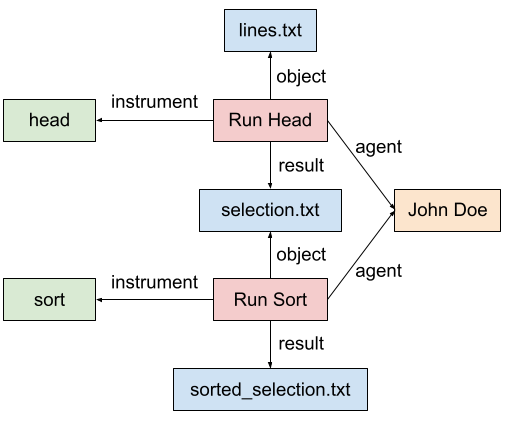
\includegraphics[width=22em]{image3.png}
\caption{{\bf Entity-Relationship diagram for Workflow Run Crate.}
The main differences with Process Run Crate are the representation of formal parameters and the fact that the application is expected to be a workflow.}
\label{fig:workflow_crate_er}
\end{figure}


\subsection{Provenance Run Crate}\label{provenance-run-crate}

The Provenance Run Crate profile extends Workflow Run Crate by adding specifications on how to describe the internal details of the workflow execution, including individual tool executions, intermediate outputs and related parameters.
Individual tool executions are represented by additional \emph{CreateAction} instances that refer to the tool itself via \emph{instrument} -- analogously to its use in Process Run Crate.
The workflow is required to refer to the tools it orchestrates through the \emph{hasPart} property, in line with recommendations from the Bioschemas ComputationalWorkflow profile.

To represent the logical steps defined by the workflow, this profile introduces the usage of \emph{HowToStep} i.e., “A step in the instructions for how to achieve a result” (\url{https://schema.org/HowToStep}).
Steps point to the corresponding tools via the \emph{workExample} property and are referenced from the workflow via the \emph{step} property; the execution of a step is represented by a \emph{ControlAction} pointing to the
\emph{HowToStep} via \emph{instrument} and to the \emph{CreateAction}
instance(s) that represent the corresponding tool execution(s) via
\emph{object}.
Note that a step execution does not coincide with a tool execution: an example where this distinction is apparent is when a step maps to multiple executions of the same tool over a list of inputs (the "scattering" feature in CWL).

An RO-Crate following this profile can also represent the execution of the WMS itself (e.g., cwltool, Nextflow~\cite{Di Tommaso 2017}) via
\emph{OrganizeAction}, pointing to a representation of the WMS via
\emph{instrument}, to the steps via \emph{object} and to the workflow run via \emph{result}.
The \emph{object} attribute of the
\emph{OrganizeAction} can additionally point to a configuration file containing a description of the settings that affected the WMS's behaviour during the execution.

Fig~\ref{fig:provenance_crate_er} shows the various entities involved in the representation of a workflow run via Provenance Run Crate together with their relationships.

\begin{figure}[!h]
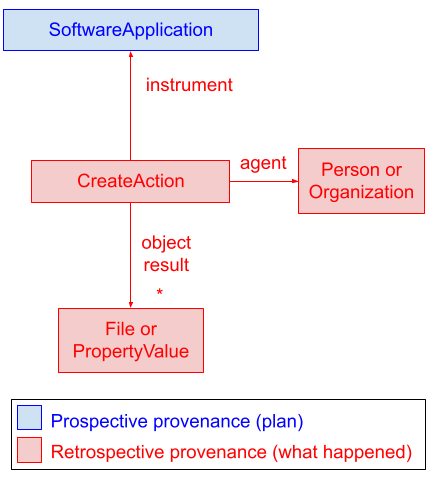
\includegraphics[width=21em]{image4.png}
\caption{{\bf Entity-Relationship diagram for Provenance Run Crate.}
In addition to the workflow run, this profile represents the execution of individual steps and their related tools.}
\label{fig:provenance_crate_er}
\end{figure}

This profile also includes specifications on how to describe connections between parameters.
Parameter connections -- a fundamental feature of computational workflows -- describe (i) how tools take as input the intermediate outputs generated by other tools and (ii) how workflow-level parameters are mapped to tool-level parameters.
For instance, in the workflow pictured in Fig~\ref{fig:revsort}, the output of the \emph{rev} step is used as one of the inputs for the \emph{sorted}
step.

\begin{figure}[!h]
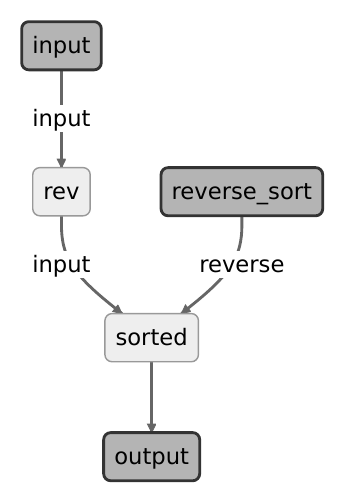
\includegraphics[width=12em]{image5.png}
\caption{{\bf Diagram of a simple workflow}
that reverses each line of the input file and then sorts the resulting stream.
The workflow connects the output parameter of the ``rev'' tool to the input parameter of the ``sort'' tool.
Provenance Run Crate provides a formalism to represent such connections.}
\label{fig:revsort}
\end{figure}

A representation of parameter connections is particularly useful for traceability, since it allows to document the inputs and tools on which workflow outputs depend.
Since the current RO-Crate context has no suitable terms for the description of such relationships, 
we added appropriate ones to the aforementioned  "workflow-run" context extension (namespace \url{https://w3id.org/ro/terms/workflow-run}):
a \emph{ParameterConnection} type with
\emph{sourceParameter} and \emph{targetParameter} attributes that respectively map to the source and target formal parameters, and a
\emph{connection} property to link from the relevant step or workflow to the \emph{ParameterConnection} instances.



%%
\section{Implementations}\label{implementations}

Support for the Workflow Run RO-Crate profiles presented in this work has been implemented in a number of systems, showing support from the community and already demonstrating a degree of usability in practice.
All these implementations are described in the following sections.


\subsection{Runcrate}\label{runcrate}

Runcrate \cite{Leo 2023a} is a generic Workflow Run RO-Crate toolkit which also serves as a reference implementation of the proposed profiles.
It consists of a Python package with a nested command line interface, providing a straightforward path to integration in Python software and other workflows.
The runcrate toolkit includes functionality to convert CWLProv ROs to RO-Crates conforming to the Provenance Run Crate profile (\emph{runcrate convert}), effectively providing an indirect implementation of the format for cwltool.
Indeed, the CWLProv model provided a basis for the Provenance Run Crate profile, and the implementation of a conversion tool in runcrate at times drove the improvement and extension of the profile as new requirements or gaps in the old designs emerged.
Runcrate converts both the retrospective provenance part of the CWLProv RO (the RDF graph of the workflow's execution) and the prospective provenance part (the CWL files, including the workflow itself).
Both parts are thus converted into a single, workflow language-agnostic metadata resource.

Another functionality offered by the runcrate package is \emph{runcrate report} which reports on the various executions described in an input RO-Crate, listing their starting and ending times, the values of the various parameters, etc.
Runcrate report demonstrates how the provenance profiles presented in this work enable comparison of runs interoperably across different workflow languages or different implementations of the same language.

We also added a \emph{run} subcommand to re-execute the computation described by an input Workflow Run Crate or Provenance Run Crate where CWL was used as a workflow language.
It works by mapping the RO-Crate description of input parameters and their values (the workflow's
\emph{input} and the action's \emph{object}) to the format expected by CWL, which is then used to relaunch the workflow on the input data.
This functionality shows the machine-actionability of the profiles to support reproducibility, and was used to successfully re-execute the digital pathology annotation workflow described in section \nameref{exemplary-use-cases}.
Of course, achieving a full re-execution in the general case may not always be possible: reproducibility is supported by the profiles, but also benefits from the characteristics of the workflow language (which should provide a clear formalism to map input items to their corresponding parameter slots) and from cooperation on the part of the workflow's author, who can help considerably by containerizing the environment required by each step and providing the relevant annotations (if allowed by the workflow language).

In order to assess runcrate, we performed a qualitative analysis of the tool's \emph{convert} mode, in which we evaluated how the generated RO-Crates preserve the metadata contained in the CWLProv ROs from which they are derived.
For this analysis, we followed the same approach as for an earlier evaluation of CWLProv~\cite{De Wit 2022}.
We distinguished three levels of representation:
firstly, in RDF; secondly, in a structured, but CWL-specific document;
and finally, in an unstructured, non-machine-accessible format.
The analysis concluded that the CWLProv RDF representation of the workflow runs was relatively sparse, even though much of the provenance metadata was contained in CWL-specific documents, such as the packed workflow and input parameter file.
We compared the CWLProv RDF provenance graph with the RO-Crate metadata file.
Because runcrate only generates RO-Crates \emph{after} workflow execution, we only considered components that in CWLProv were at least partially represented in structured format (CWL-specific or RDF), and analyzed their presence in RDF in RO-Crate (the packed CWL workflow is identical between CWLProv and RO-Crate).

The results of the analysis are summarised in Table
\cite{analysis\_table}.
Overall, most of the information contained in CWLProv RDF is transferred to the RO-Crate metadata.
In addition, the representation of some categories of metadata has improved, notably Workflow parameters (WF2), which were insufficiently described in CWLProv RDF but defined with type and format in RO-Crate.
Moreover, the format of input files (D2), which was absent in CWLProv RDF, is represented in RO-Crate.
One aspect in which RO-Crate RDF is sparser than CWLProv is computational environment (T5): whereas in CWLProv names of container images were preserved (ENV3), this information is not carried over to the RO-Crate metadata file in the current runcrate version, as the representation of container images in the profiles is under discussion.
It should be noted, however, that reproducibility is still supported by the presence of container image information in the CWL workflow file included in the RO-Crate.

In conclusion, our analysis shows that runcrate preserves most provenance metadata previously shown to be relevant in realistic RO use case scenarios.
The full results of the analysis can be found at \url{https://github.com/RenskeW/runcrate-analysis}.


% Place tables after the first paragraph in which they are cited.
\begin{table}[!ht]
\begin{adjustwidth}{-1.4cm}{0in} % Comment out/remove adjustwidth environment if table fits in text column.
\centering
\caption{
{\bf Summarised results of our qualitative analysis of runcrate.}}
\begin{tabular}{r|l|l|c|c|c}
\hline
%% TODO: Check ticks are in right places
{\bf Type} & {\bf Subtype} & {\bf Name} & {\bf CWL} & {\bf CWLProv} & {\bf RO-Crate} \\ \thickhline
T1 & SC1 & Workflow design & f & &\\ 
& SC2 & Entity annotations & p & &\\ 
& SC3 & Workflow execution annotations * & & &\\ \hline
T2 & D1 & Data identification & p & & \\
& D2 & File characteristics & p & p & p \\
& D3 & Data access & p & & \\ 
& D4 & Parameter mapping & f & f & f \\ \hline 
T3 & SW1 & Software identification & p & & \\ 
& SW2 & Software documentation & p & & \\  
& SW3 & Software access & p & & \\ \hline 
T4 & WF1 & Workflow software metadata & f & p & p\\ 
& WF2 & Workflow parameters & f & p & p \\ 
& WF3 & Workflow requirements & f & & \\ \hline 
T5 & ENV1 & Software environment * & & & \\ 
& ENV2 & Hardware environment * & & &\\ 
& ENV3 & Container image & p & p & \\ \hline 
T6 & EX1 & Execution timestamps & f & f &\\ 
& EX2 & Consumed resources * & & & \\ 
& EX3 & Workflow engine & p & f & \\  
& EX4 & Human agent & f & f & \\ \hline
\end{tabular}
\begin{flushleft} We compared RO-Crates with the CWLProv ROs from which they were generated.
The analysis was based on a provenance taxonomy reflecting relevant provenance metadata based on realistic use cases for ROs associated with a real-life bioinformatics workflow.
We only considered provenance metadata which was already represented in CWLProv RDF or CWL-specific documents (packed.cwl, primary-job.json, and primary-output.json).
Since packed.cwl is also included in RO-Crate, we only considered how the metadata was represented in ro-crate-metadata.json.\\
\textbf{Legend:} p = partially represented, f = fully represented. * = missing or unstructured representation in CWLProv
\end{flushleft}
\label{analysis_table}
\end{adjustwidth}
\end{table}


\subsection{Galaxy}\label{galaxy}

The Galaxy project~\cite{Jalili 2020} provides a WMS with data management functionalities as a multi-user platform, aiming to make computational biology more accessible to research scientists that do not have computer programming or systems administration experience.
Galaxy's most prominent features include: a collection of 7500+ integrated tools (\url{https://galaxyproject.org/toolshed/});
a web interface that allows the execution and definition of workflows using the integrated tools; a network of dedicated (public) Galaxy instances.

The export of workflow execution provenance data as Workflow Run Crates has been added in Galaxy's 23.0 release.
This feature provides a more interoperable alternative to the basic export of Galaxy workflow
\emph{invocations}: the workflow definition; a set of serialisations of the invocation-related metadata in Galaxy native, json-formatted files;
and the input and output data files.
This is achieved by extracting provenance from Galaxy entities related to the workflow run, along with associated metadata, converting them to RO-Crate metadata using the ro-crate-py library~\cite{De Geest 2022}; by describing all files contained in the basic invocation export within the RO-crate metadata;
and finally by making the Workflow Run Crate available for export to the user through Galaxy's web interface and API.

We extract the prospective provenance contained in Galaxy's YAML-based gxformat2
(\url{https://galaxyproject.github.io/gxformat2/v19_09.html}) workflow definition, which includes details of the analysis pipeline such as the graph of tools that need to be executed, and metadata about the data types required.
The retrospective provenance -- i.e., the details of the executed workflow such as the inputs, outputs, parameter values used -- is extracted from Galaxy's data model (\url{https://docs.galaxyproject.org/en/master/lib/galaxy.model.html}), which is not directly accessible to users in the context of a public Galaxy server.
All of this provenance information is then mapped to RO-Crate metadata, including some Galaxy-specific data entities such as dataset collections.
An exemplary exported Galaxy Workflow Run Crate is made available on Zenodo~\cite{De Geest 2023}.

In practice, a user would take the following steps to obtain a Workflow Run Crate from a Galaxy instance: 1) create or download a Galaxy workflow definition (e.g.: from WorkflowHub) and import it in a Galaxy instance, or create a workflow through the Galaxy GUI directly; 2) execute the workflow, providing the required inputs; 3) after the workflow has run successfully, the corresponding RO-Crate will be available for export from the Workflow Invocations list.

Future work includes adding metadata detailing each step of the workflow run to conform to the Provenance Run Crate profile; developing and/or integrating RO-Crate more deeply with import and export of Galaxy histories through the implementation of a profile; further developing features to allow for user-guided import of RO-Crates as Galaxy datasets, histories and workflows.

\subsection{COMPSs}\label{compss}

COMPSs~\cite{Lordan 2014} is a task-based programming model that allows users to transform a sequential application into a parallel one by simply annotating some of its methods, thus making it efficient to exploit the resources available (either distributed or in a cluster).
When a COMPSs application is executed, a corresponding workflow describing the application's tasks and their data dependencies is dynamically generated and used by the COMPSs runtime to orchestrate the execution of the application in the infrastructure.
As a WMS, COMPSs stands out for its many advanced features that enable applications to achieve fine-grained high efficiency in HPC systems, such as the ability to exploit underlying parallelisation frameworks (i.e.~MPI, OpenMP), compilers (e.g.~NUMBA), failure management, task grouping, and more.

Provenance recording for COMPSs workflows has been explored in previous work~\cite{Sirvent 2022}, where the Workflow RO-Crate profile was adopted in the implementation of a very lightweight approach to document provenance while avoiding the introduction of any significant run time performance overheads.
However, because of the dynamic nature of COMPSs workflows, the Workflow Run Crate profile is better suited to represent them, since workflows are created when the application is executed and, thus, a prior static workflow definition does not exist before that moment.
Due to this limitation, the workflow entity in the metadata file references the entry point application run by COMPSs, and formal parameters are not listed (note that listing them is not required by the profile) because inputs and outputs (both for each task and the whole workflow) are determined at runtime.
COMPSs is able to export provenance data with a post-processing operation that can be triggered at any moment after the application has finished.
The RO-Crate generation post-process uses information recorded by the runtime to detect and automatically add metadata of any input or output data assets used by the workflow.

Implementing Workflow Run Crate support in COMPSs required particular attention to the generation of a unique id for the \emph{CreateAction} representing the workflow run, combining hostname and queuing system job id for supercomputer executions, and using generated UUIDs for distributed environments, to add as much as information available from the run while ensuring the id is unique.
In the \emph{CreateAction}, the \emph{description} term includes system information, as well as relevant environment variables that provide details on the execution environment (e.g., node list, CPUs per node).
Finally, a reference to the system's monitoring tool (when available) is also included in the \emph{subjectOf} clause, where authorised users can see detailed profiling of the corresponding job execution, as provided by MareNostrum IV supercomputer (\url{https://bsc.es/supportkc/docs/MareNostrum4/intro/}).

To showcase the COMPSs adoption of the Workflow Run Crate profile, we provide as an example the execution of the BackTrackBB~\cite{Poiata 2016}
application in the MareNostrum IV supercomputer.
BackTrackBB targets the detection and location of seismic sources using the statistical coherence of the wave field recorded by seismic networks and antennas.
The resulting RO-Crate~\cite{Poiata 2023} complies with the Workflow Run Crate profile, and includes the application source files, a diagram of the workflow's graph, application profiling and input and output files.

The implementation of provenance recording following Workflow Run Crate has been fully integrated in the COMPSs runtime, and is available since release 3.2 (May 2023).


\subsection{StreamFlow}\label{streamflow}

The StreamFlow framework~\cite{Colonnelli 2020} is a container-native WMS based on the CWL standard.
It has been designed around two primary principles: first, it allows the execution of tasks in multi-container environments, supporting the concurrent execution of communicating tasks in a multi-agent ecosystem; second, it relaxes the requirement of a single shared data space, allowing for hybrid workflow executions on top of multi-cloud, hybrid cloud/HPC, and federated infrastructures.
StreamFlow orchestrates hybrid workflows by combining a \emph{workflow description} (e.g., a CWL workflow description and a set of input values) with one or more \emph{deployment descriptions} -- i.e.
representations of the execution environments in terms of infrastructure-as-code (e.g., Docker Compose files, HPC batch scripts, and Helm charts).
A streamflow.yml file -- the entry point of each StreamFlow execution -- binds each workflow step with the set of most suitable execution environments.
At execution time, StreamFlow automatically takes care of all the secondary aspects, like scheduling, checkpointing, fault tolerance, and data movements.

StreamFlow stores provenance data in a proprietary format into a persistent pluggable database (using sqlite3 as the default choice).
After a CWL workflow execution completes, users can generate an RO-Crate through the streamflow prov \textless workflow\_name\textgreater{}
command, which extracts the provenance data stored in the database for one or more workflow executions and converts it to an RO-Crate archive that is fully compliant with the Provenance Run Crate Profile, including the details of each task run by the WMS.
The StreamFlow configuration and a description of the hybrid execution environment are preserved by directly including the streamflow.yml file into the generated archive.
Support for the format has been integrated into the main development branch and will be included in release 0.2.0.

\subsection{WfExS}\label{wfexs}

WfExS-backend (\url{https://github.com/inab/WfExS-backend}) is a FAIR workflow execution service that aims to address some of the difficulties found in analysing sensitive data in a secure manner.
The WfExS-backend delegates the actual workflow execution to a specific workflow manager (e.g., Nextflow or cwltool).
WfExS-backend fetches and materialises all the elements needed to run a workflow -- i.e.~the workflow itself, the WMS, the required software containers and the inputs.
Of note, the orchestrator can consume RO-Crates from WorkflowHub to import workflows to be executed.

Support has been added to the WfExS-backend to export provenance data as RO-Crates following the Workflow Run Crate profile, which has proven to be a mechanism suitable to semantically describe digital objects in a way that simplifies embedding key details involved in analysis reproducibility and replicability.

The WfExS-backend records details relevant to the prospective provenance when a workflow is prepared for execution, such as the public URIs used to fetch input data and workflows, fingerprints, and metadata derived from workflow files, container images and input files.
WfExS-backend has explicit commands to generate both prospective and retrospective provenance RO-Crates.
If a workflow is executed more than once in the very same staged directory, run details from all the executions are represented in the retrospective provenance RO-Crate.
Future developments will also add support for embedding URIs of output results that have been published to a suitable repository (like Zenodo DOIs, for instance).

\subsection{Sapporo}\label{sapporo}

Sapporo~\cite{Suetake 2022a} is an implementation of the Workflow Execution Service (WES) API specification \cite{Magee 2018}.
WES is a standard proposed by the Global Alliance for Genomics and Health (GA4GH) for cloud-based data analysis platforms that receive requests to execute workflows.
Sapporo supports the execution of several workflow types, including cwltool \cite{Amstutz 2023}, Toil \cite{Vivian 2017}, and StreamFlow \cite{Colonnelli 2020}.
Sapporo includes features specifically tailored to bioinformatics applications, including the calculation of feature statistics from specific types of outputs generated by workflow runs.
For example, the system calculates the mapping rate of DNA sequence alignments from BAM format files.
To describe the feature values, Sapporo uses the Workflow Run Crate profile extended with additional RO terms to represent these biological features.

Further, the Tonkaz companion command line software has integrated functionality to compare Run Crates generated by Sapporo to measure the reproducibility of the workflow outputs~\cite{Suetake 2022b}.
Developers can use this unique feature to build a CI/CD platform for their workflows to ensure that changes to the product do not produce an unexpected result.
Workflow users can also use this feature to verify the results from the same workflow deployed in different environments.

While Sapporo supports Workflow Run Crate, since WES is a WMS wrapper, it does not parse the provided workflow definition files. 
Instead, it embeds the information in the files passed by the WES request to record the provenance of execution rather than using the actual workflow parameters meant for the wrapped WMS.
Therefore, the current implementation of Sapporo does not capture the connections between the inputs/outputs depicted in the workflow and the actual files used/generated during the run.
Thus, the profile generated by Sapporo has fields representing input and output files, but they are not linked to formal parameters.

\subsection{Autosubmit}\label{autosubmit}

Autosubmit~\cite{Manubens-Gil 2016} is an open source lightweight workflow manager and meta-scheduler created in 2011 for use in climate research to configure and run scientific experiments.
It supports scheduling jobs via SSH to Slurm, PBS and other remote batch servers used in HPC.

The ``archive'' feature was added in Autosubmit 3.1.0, released in 2015.
This feature archives the experiment directory and all its contents into a ZIP file, which can be used later to access the provenance data or to execute the Autosubmit experiment again.
Even though the data in the ZIP file includes prospective provenance and retrospective provenance, it contains no structure, and users have no way to tell which is which from just looking at the ZIP file and its contents.

Recent releases of Autosubmit 4 include an updated YAML configuration management system that allows users to combine multiple YAML files into a single unified configuration file.
While this gave users flexibility, it also increased the complexity to track the configuration changes and to relate these to the provenance data.

Another feature added in Autosubmit 4 was the option to use only the experiment manager features of Autosubmit, delegating the workflow execution to a different backend workflow engine, like ecFlow~\cite{Bahra 2011}, Cylc~\cite{Oliver 2023}, or a CWL runner.

In order to give users a more structured way to archive provenance, which includes the complete experiment configuration and the parameters used to generate the unified experiment configuration, and also to allow interoperability between workflow managers, the archive feature received a new flag to generate Workflow Run RO-Crates instead of plain ZIP files.

The prospective provenance data is extracted from the Autosubmit experiment configuration.
This includes the multiple YAML files, and the unified YAML configuration, as well as the parameters used to preprocess each file --- preprocessing replaces placeholders in script templates with values from the experiment configuration.
The retrospective provenance data is included with the RO-Crate archive and includes logs and other traces produced by the experiment workflow.
Both prospective and retrospective provenance data are included in the final RO-Crate JSON-LD metadata file.

As one of the most recent implementations, much of the code added in Autosubmit 4 for RO-Crates was adapted from existing implementations like COMPSs and StreamFlow.
ro-crate-py~\cite{De Geest 2022} was used for the heavy lifting work of creating the RO-Crate archive in Python, and adding information for the JSON-LD metadata.

The main challenges for adopting RO-Crate in Autosubmit were incorporating Autosubmit's ``Project'' feature, and the lack of validation tools and of documentation and examples on how to use the standard with \emph{coarse-grained} workflow management systems (as described in~\cite{Goble 2020}) that do not track inputs and outputs, which is the case of Autosubmit --- as well as Cylc and ecFlow.

A Project in Autosubmit is an abstract concept that has a type and a location.
The type can be Git, Subversion, or Local.
For each type the location represents the URL of a code repository, or a directory on a workstation or HPC file system used to copy the Project and its template scripts (written in Shell, R, or Python) and any other files (input data for a model, extra configuration files, binaries, etc.).
The workflows in Autosubmit have tasks with dependencies to other tasks, and each of these tasks execute one of these template scripts.
The RO-Crate archive generated by Autosubmit includes only the project type and location, and not the complete Project.
This means users have the provenance of the Project, but only those with the correct permissions can access its constituent resourcesit (many applications run with Autosubmit can not be publicly shared without consent).

Validation tools for RO-Crate archives are still under development, and while there is a community-based review process to help and guide new implementations, a tool that others can use as code is written will contribute to a more agile development.

After working with the RO-Crate community on these issues, the Autosubmit team adopted a mixed approach where Autosubmit initialises the JSON-LD metadata from its configuration and local trace files, and the user is responsible for providing a partial JSON-LD metadata object in the Autosubmit YAML configuration.
A pull request was created to ro-crate-py to allow the RO-Crate JSON-LD metadata to be patched by these partial JSON-LD metadata objects.
This way, users are able to provide the missing information from the Autosubmit configuration model, like licence, authors, inputs, outputs, formal parameters, and more.
And by modifying ro-crate-py, future implementers of RO-Crate that have a similar workflow configuration as Autosubmit should be able to re-use it, while also using COMPSs, StreamFlow, Autosubmit, and other implementations as reference.

A workflow was created using an example Autosubmit Project~\cite{Kinoshita 2023} designed using UFZ's mHM (mesoscale Hydrological Model)
\cite{Samaniego 2010,Kumar 2013} to validate the RO-Crate produced by Autosubmit.

Table \ref{implementation_summary_table} shows an overview of the different profiles presented in this section, with their corresponding version URL and examples used for profile and implementation validation.

\begin{table}[!ht]
  \begin{adjustwidth}{-1.4cm}{0in} % Comment out/remove adjustwidth environment if table fits in text column.
  \centering
  \caption{
  {\bf Workflow Run Crate implementation}}
  \begin{tabular}{l|l|l|l}
  \hline
  {\bf Implementation} & {\bf WF Run RO-Crate Profile} & {\bf Version URL/DOI} &
  {\bf Example}\\
  \thickhline
  runcrate & Process, Workflow, Provenance & &\\
  Galaxy & Provenance, Workflow & & \\
  COMPSs & Provenance, Workflow & & \\
  Streamflow & \ldots{} & & \\
  WfExS & & & \\
  Sapporo & & & \\
  Autosubmit & Provenance, Workflow & & \cite{Kinoshita 2023} \\

  \end{tabular}
  \begin{flushleft} 
    Summary of each implementation together with the profiles it implements, the latest version URL/DOI and an example used for validation.
  \end{flushleft}
  \label{implementation_summary_table}
  \end{adjustwidth}
  \end{table}
  


%% 
\section{Exemplary Use Cases}\label{exemplary-use-cases}

We evaluate illustrate Workflow Run RO-Crate on two exemplary use cases, which are similar in terms of application domain -- machine learning-aided tumour detection in human prostate images -- but quite different in the way computations are executed and provenance is represented: in the first, the analysis is conducted by means of a CWL workflow and the outcome is represented with Provenance Run Crate; in the second, a combination of Process Run Crate and CPM RO-Crate is used to represent a sequence of computations linked to their corresponding CPM provenance information.


\subsection{Provenance Run Crate for Digital Pathology}\label{provenance-run-crate-for-digital-pathology}

We present a use case that demonstrates the effectiveness of Provenance Run Crate at recording provenance data in the context of digital pathology.
More specifically, we demonstrate the generation of RO-Crates to save provenance data associated with the computational annotation of magnified prostate tissue areas and cancer subregions using deep learning models~\cite{Del Rio 2022}.
The image annotation process is implemented in a CWL workflow consisting of three steps, each executing inference on an image using a deep learning model: inference of a low-resolution tissue mask to select areas for further processing;
high-resolution tissue inference on areas identified in the previous step to refine borders; high-resolution cancer identification on areas identified in the first step.
The two tissue inference steps run the same tool, but set different values for the parameter that controls the magnification level.
The workflow is integrated in the CRS4 Digital Pathology Platform (\url{https://github.com/crs4/DigitalPathologyPlatform}), a web-based platform to support clinical studies involving the examination and/or the annotation of digital pathology images.

Using the same exemplary workflow, we implemented provenance recording on two different execution platforms.
In the first case, the workflow was executed with the StreamFlow WMS, for which the Provenance Run Crate implementation is discussed in Section \nameref{provenance-run-crate}.
In the second case, we executed the CWL workflow with cwltool and converted the resulting CWLProv RO to a Provenance Run Crate with the runcrate tool (section \nameref{runcrate}).

The RO-Crates obtained in the two cases~\cite{Colonnelli 2023, Leo 2023b}
are very similar to each other, differing only in a few details: for instance,~\cite{Colonnelli 2023} includes the StreamFlow configuration file and has separate files for the workflow and the two tools, while
\cite{Leo 2023b} has the workflow and the tools stored in a single file (CWL's "packed" format).
Apart from these minor differences, the description of the computation is essentially the same.
Four actions are represented: the workflow itself, the two executions of the tissue extraction tool and the execution of the tumour classification tool.
Each action is linked to the corresponding workflow or tool via the
\emph{instrument} property, and its starting and ending time are recorded; for each action, input and output slots are referenced by the workflow, while the corresponding values are referenced by the action itself.
The data entities and \emph{PropertyValue} instances corresponding to the input and output values link to the corresponding parameter slots via the \emph{exampleOfWork} property, providing information on the values taken by the parameters.
The listing below shows the output of the
\emph{runcrate report} command for the StreamFlow RO-Crate.

\begin{adjustwidth}{-1.5cm}{0in}
\label{lst:ml_pipeline_streamflow_report}
\begin{verbatim}
action: #30a65cba-1b75-47dc-ad47-1d33819cf156
  instrument: predictions.cwl (['SoftwareSourceCode', 
         'ComputationalWorkflow', 'HowTo', 'File'])
  started: 2023-05-09T05:10:53.937305+00:00
  ended: 2023-05-09T05:11:07.521396+00:00
  inputs:
    #af0253d688f3409a2c6d24bf6b35df7c4e271292 <- predictions.cwl#slide
    tissue_low <- predictions.cwl#tissue-low-label
    9 <- predictions.cwl#tissue-low-level
    tissue_low>0.9 <- predictions.cwl#tissue-high-filter
    tissue_high <- predictions.cwl#tissue-high-label
    4 <- predictions.cwl#tissue-high-level
    tissue_low>0.99 <- predictions.cwl#tumor-filter
    tumor <- predictions.cwl#tumor-label
    1 <- predictions.cwl#tumor-level
  outputs:
    06133ec5f8973ec3cc5281e5df56421c3228c221 <- predictions.cwl#tissue
    4fd6110ee3c544182027f82ffe84b5ae7db5fb81 <- predictions.cwl#tumor

action: #457c80d0-75e8-46d6-bada-b3fe82ea0ef1
  step: predictions.cwl#extract-tissue-low
  instrument: extract_tissue.cwl (['SoftwareApplication', 'File'])
  started: 2023-05-09T05:10:55.236742+00:00
  ended: 2023-05-09T05:10:55.910025+00:00
  inputs:
    tissue_low <- extract_tissue.cwl#label
    9 <- extract_tissue.cwl#level
    #af0253d688f3409a2c6d24bf6b35df7c4e271292 <- extract_tissue.cwl#src
  outputs:
    6b15de40dd0ee3234062d0f261c77575a60de0f2 <- extract_tissue.cwl#tissue

action: #d09a8355-1a14-4ea4-b00b-122e010e5cc9
  step: predictions.cwl#extract-tissue-high
  instrument: extract_tissue.cwl (['SoftwareApplication', 'File'])
  started: 2023-05-09T05:10:58.417760+00:00
  ended: 2023-05-09T05:11:03.153912+00:00
  inputs:
    tissue_low>0.9 <- extract_tissue.cwl#filter
    6b15de40dd0ee3234062d0f261c77575a60de0f2 <- extract_tissue.cwl#filter_slide
    tissue_high <- extract_tissue.cwl#label
    4 <- extract_tissue.cwl#level
    #af0253d688f3409a2c6d24bf6b35df7c4e271292 <- extract_tissue.cwl#src
  outputs:
    06133ec5f8973ec3cc5281e5df56421c3228c221 <- extract_tissue.cwl#tissue

action: #ae2163a8-1a2a-4d78-9c81-caad76a72e47
  step: predictions.cwl#classify-tumor
  instrument: classify_tumor.cwl (['SoftwareApplication', 'File'])
  started: 2023-05-09T05:10:58.420654+00:00
  ended: 2023-05-09T05:11:06.708344+00:00
  inputs:
    tissue_low>0.99 <- classify_tumor.cwl#filter
    6b15de40dd0ee3234062d0f261c77575a60de0f2 <- classify_tumor.cwl#filter_slide
    tumor <- classify_tumor.cwl#label
    1 <- classify_tumor.cwl#level
    #af0253d688f3409a2c6d24bf6b35df7c4e271292 <- classify_tumor.cwl#src
  outputs:
    4fd6110ee3c544182027f82ffe84b5ae7db5fb81 <- classify_tumor.cwl#tumor
\end{verbatim}
\end{adjustwidth}



The \emph{exampleOfWork} link between input / output values and parameter slots is used by \emph{runcrate run} to reconstruct the CWL input parameters document needed to rerun the computation.
The
\emph{alternateName} property (a Schema.org property applicable to all entities), which records the original name (i.e., at the time the computation was run) of data entities, is also crucial for reproducibility in this case: both StreamFlow and CWLProv, to avoid clashes, record input and output files and directories using their SHA1
checksum as their names. 
However, this particular workflow expects the input dataset to be in the MIRAX (\url{https://openslide.org/formats/mirax/}) format, where the "main" file taken as an input parameter by the processing application must be accompanied by a directory in the same location with the same name apart from the extension.
The runcrate tool uses the \emph{alternateName} to rename the input dataset as required, so that the expected pattern can be picked up by the workflow during the re-execution.
This use case was the main motivation to include a recommendation to use alternateName with the above semantics in Process Run Crate.

Thanks to the fact that both RO-Crates were generated following the best practices to support reproducibility mentioned in the profiles, we were able to re-execute both computations with the runcrate tool.
This was also made possible by the inclusion of the information on which container images to use for each tool in the CWL workflow.
Overall, this shows how reproducibility is a hard-to-achieve goal that can only be supported, but not ensured, by the profiles, since it also depends on factors like the characteristics of the computation, the choice of workflow language and whether best practices such as containerization are followed.

This use case highlighted the need to add specifications on how to represent multi-file datasets \cite[section Representing multi-file objects]{Workflow Run RO-Crate working group 2023a}. In the MIRAX format, in fact, the "main" file must be accompanied by a directory in the same location containing additional files with a specific structure.

\subsection{Process Run Crate and CPM RO-Crate for cancer detection}\label{process-run-crate-and-cpm-ro-crate-for-cancer-detection}

This section presents an RO-Crate created to describe an execution of a computational pipeline that trains AI models to detect the presence of carcinoma cells in high-resolution digital images of magnified human prostate tissue.
The pipeline consists of three main computational steps: a preprocessing step that splits input images into small patches and divides them into a training and a testing set; a training step that trains the model to recognize the presence of carcinoma cells in the images; an evaluation step that measures the accuracy of the trained model on the testing set.

In addition to the pipeline steps, the RO-Crate describes additional computations related to the generation of the CPM provenance and meta-provenance files.
All computations are described according to the Process Run Crate profile, while the CPM files are referenced according to the CPM RO-Crate profile (section \nameref{synergy-with-the-cpm-ro-crate-profile}).
Also represented via Process Run Crate are: the input dataset; the results of the pipeline execution; the scripts that implement the pipeline; the log files generated by the scripts; a script that converts the logs into the CPM files.
This allowed us to describe all involved elements as a single aggregate, with entities and their relationships represented according to the RO-Crate model.
The RO-Crate discussed here is available from Zenodo~\cite{Wittner 2023}.

The CPM files complement the RO-Crate with internal details about the pipeline execution, such as how the input dataset was split into training and testing sets, or detailed information about each training iteration of the AI model.
For instance, the entity \texttt{ns\_training:modelIter2} present in the \texttt{ns\_training:bundle\_training} bundle represents a checkpoint of the AI model after the second training iteration.
The entity's attributes contain paths to the respective model stored as a file.
The entity is related to the respective training iteration activity \texttt{ns\_training:trainIter1}, which contains the iteration parameters represented as an attribute list.
In addition, the CPM generally provides means to link the input dataset provenance to the provenance of its precursors -- human prostate tissues and biological samples the tissues were derived from; this is not included in the example because we used a publicly available input database for which provenance of the precursors was not available.
However, the linking mechanism for provenance precursors is exactly the same as between the bundles for the AI pipeline parts.
While the RO-Crate is focused on the execution of the pipeline, the provenance included in the CPM files intends to be interlinked with provenance of the precursors or successors, providing means to traverse the whole provenance chain.
As a result, combining the CPM and RO-Crate enables the lookup of research artefacts related to the computation across heterogeneous organisations using the underlying provenance chain.

Differences between CPM and Process Run Crate content, in general:

\begin{itemize}
  \item 
CPM focused on traceability of inputs/outputs in a distributed(multi-organizational) environments. What is considered an input/output in Process Run Crate might not be relevant for the CPM and vice versa. For instance, a configuration file is probably not an input for a script, because I am not interested in history of the config in a sense that I would trace its provenance back to its source.
\item CPM probably more general – can be applied to describe both physical and digital objects. 
\item In CPM based files, you may add arbitrary domain specific information represented as an arbitrary provenance graph connected to provenance chain in a prescribed way. I am not sure whether I can add my own relations into the crate, if they are not defined by the profile. 
\end{itemize}


%
\section{Discussion}\label{discussion}


The RO-Crate profiles presented here provide a unified data model to describe the prospective and retrospective provenance of the execution of a computational workflow, together with contextual metadata about the workflow itself and its associated entities (inputs, outputs, code, etc.). 
The profiles are flexible, allowing to tailor the description to a broad variety of use cases, agnostic with respect to the WMS used and allow describing provenance traces at different levels of granularity. 
This facilitates developing implementations by multiple workflow systems (often with heterogeneous assumptions and requirements) -- six of which have already been developed and are described in Section \nameref{implementations} -- allowing to perform comparisons between runs across heterogeneous systems.
Additionally, having workflow runs and plans described according to the RO-Crate model allows to capture the context of the workflow itself (e.g.~authors, related publications, other workflows, etc.) rather than the trace alone. 
Being based on RO-Crate, the profiles and their implementations are part of a growing ecosystem of tools and services maintained by the RO-Crate community (\url{https://www.researchobject.org/ro-crate/in-use/}).
The Workflow Run Crate and Provenance Run Crate profiles are also compatible with the WorkflowHub registry, allowing workflow runs created with those profiles to be registered and easily found and shared with other researchers.


In the introduction, we have provided background on computational provenance representation, focusing on CWLProv as the present work is, in part, an effort to overcome its limitations.
A project that uses Bagit-serialized ROs similar to those used by CWLProv is Whole Tale
\cite{Chard 2019}, a web platform with a focus on the narrative around scientific studies and their reproducibility, where the serialized ROs are used to export data and metadata from the platform.
In contrast, our work is primarily focused on the RO-Crate profiles and their ability to capture the provenance of computational workflow execution.

The Workflow Run RO-Crate profiles, the associated tooling, the implementations and the examples are developed by a community that runs regular virtual meetings (every two weeks at the time of writing) and coordinates on Slack and the RO-Crate mailing list.
The WRROC community brings together members of the RO-Crate community~\cite{Soiland-Reyes 2022a}, WMS users and developers, Workflow users and developers, GA4GH~\cite{Rehm 2021} Cloud developers and provenance model authors, and is open to anyone who is interested in the representation of workflow provenance.
The inclusion of WMS developers and workflow users was key to keeping the specifications flexible, easy to implement and grounded on real use cases, while the diversity of the stakeholders allowed to keep a plurality of viewpoints while driving the model's development forward.

One of the main benefits of this development process is that the profiles are already in use, with several implementations already available as described in section \ref{implementations}.

In the following subsections, we illustrate how the model relates to W3C PROV and to other community projects.

\subsection{Workflow Run RO-Crate and the W3C PROV standard}

Our aim is to be compatible with both Schema.org and W3C PROV. Provenance Run Crate is the profile that most closely matches the level of detail provided by CWLProv, which extends W3C PROV. Table \ref{rocrate_prov_mapping} shows how the main entities and relationships represented by Provenance Run Crate map to PROV constructs. A machine-readable version of the mapping can be found online (\textbf{TODO}).

\begin{table}[!ht]
  %\begin{adjustwidth}{-2.25in}{0in} % Comment out/remove adjustwidth environment if 
  \begin{adjustwidth}{-1.5cm}{0in}
  \centering
  \caption{
  {\bf Mapping between W3C PROV concepts and their equivalents in Workflow Run RO-Crate.}}
  \begin{tabular}{p{35mm}|p{40mm}|p{40mm}}
  \hline
  {\bf W3C PROV} & {\bf RO-Crate} & \textbf{Relationship} \\
  \thickhline
  
  \emph{activity} (workflow/ \newline process execution) 
    & \emph{CreateAction}, \emph{OrganizeAction} & Broader than \\ \hline
  \emph{agent} (WMS) & \emph{instrument} of \emph{OrganizeAction} & Equivalent \\ \hline
  \emph{agent} -- \emph{Person} & \emph{Person}  & Equivalent \\ \hline
  \emph{agent} -- \emph{Organization} & \emph{Organization}  & Equivalent \\ \hline
  \emph{agent} -- \emph{SoftwareAgent} & \emph{SoftwareApplication}  & Broader than \\ \hline
  \emph{entity} -- \emph{Plan} & 
    \emph{ComputationalWorkflow} \emph{SoftwareApplication, HowTo}  
    & Broader than \\ \hline
  \emph{entity} (other) & \emph{File}, \emph{Dataset}, \emph{PropertyValue} & Broader than \\ \hline
  \emph{wasStartedBy} & \emph{agent} and \emph{startTime} on  \emph{CreateAction} & Narrower than  \\ \hline
  \emph{wasEndedBy} & \emph{agent} and \emph{endTime} on  \emph{CreateAction} & Narrower than \\ \hline
  \emph{wasAssociatedWith} & \emph{agent} and \emph{instrument} on  \emph{CreateAction} & Broader than \\ \hline
  \emph{hadPlan} + \emph{Association} &  \emph{instrument} on \emph{CreateAction} & 
    Complex mapping: an instrument implies the existence of a qualified association (\texttt{prov:Association}) linked to a \texttt{prov:Plan} through \texttt{prov:hadPlan}
    \\ \hline
  \emph{Agent} + \emph{Association} &  \emph{agent} on \emph{CreateAction} & 
    Complex mapping: an agent implies the existence of a qualified association (\texttt{prov:Association}) linked to a \texttt{prov:Plan} through \texttt{prov:agent}
    \\ \hline  
  \emph{used} & \emph{object} on \emph{CreateAction} & Equivalent \\ \hline 
  \emph{wasGeneratedBy} & \emph{result} on  \emph{CreateAction} & Equivalent \\ \hline
  
  \end{tabular}
  %\begin{flushleft} Table notes \end{flushleft}
  \label{rocrate_prov_mapping}
  \end{adjustwidth}
\end{table}
  
    
\subsection{Synergy with the CPM RO-Crate profile}\label{synergy-with-the-cpm-ro-crate-profile}
  
The Common Provenance Model (CPM)~\cite{Wittner 2022}, an extension of the W3C PROV model~\cite{Moreau 2013}, is a recently developed provenance model that enables the representation of distributed provenance.
Distributed provenance is created when an object involved in the research process, either digital or physical (e.g., biological material), is exchanged between organisations, so that each organisation can document only a portion of the object's life cycle.
Individual provenance components are generated, stored, and managed individually by each organisation, and are linked together in a \emph{chain}.
The CPM prescribes how to represent such provenance, and how to enable its traversal and processing using a common algorithm, independently from the type of object being described.
In addition, the CPM defines a notion of meta-provenance, which contains metadata about the history of individual provenance components.

CPM RO-Crate (\url{https://w3id.org/cpm/ro-crate}) is an RO-Crate profile that supports the identification of CPM-based provenance and meta-provenance files within an RO-Crate, allowing to pack data, metadata, and CPM-based provenance information together.
An RO-Crate generated according to the CPM-RO-Crate profile embeds parts of the distributed provenance, which may be linked to the provenance of precursors and successors of the packed data.
  
The CPM-RO-Crate profile synergises well with Process Run Crate, since the former can add references to CPM-based provenance descriptions of computational executions described with the latter, integrating them in the distributed provenance.
Since CPM-based provenance and meta-provenance files are typically themselves produced by computations, Process Run Crate allows to represent these along with the main computations that produce the datasets being exchanged, providing the full picture in a cohesive ensemble.
An example of such an RO-Crate is presented in section~\cite{Process Run Crate and CPM RO-Crate}.

\subsection{Trusted Workflow Run Crate}\label{trusted-workflow-run-crate}

The TRE-FX project (\url{https://trefx.uk/}) has developed \emph{Trusted Workflow Run Crate}
(\url{https://w3id.org/trusted-wfrun-crate/0.3}), a profile that extends the Workflow Run Crate profile for use in
\emph{Trusted Research Environments} (TRE) to handle sensitive health data in federated workflow execution across TREs in the UK following the Five Safes Framework~\cite{Desai et al 2016}.

In this scenario, a crate with a workflow run request references a pre-approved workflow and project details for manual and automated assessment according to the TRE's agreement policy for the sensitive dataset.

The crate goes through multiple phases internal to the TRE, including validation, sign-off, workflow execution and disclosure control.
At this stage the crate is also conforming to the Workflow Run Crate profile.
The final crate is then safe to be made public.
This extension of Workflow Run Crate documents and supports the human review process --
important for transparency on TRE data usage.
TRE-FX is implementing this profile using WfExS as the workflow execution backend.

  

\hypertarget{conclusion}{%
\section{Conclusion}\label{conclusion}}

We presented Workflow Run RO-Crate, a collection of RO-Crate profiles to represent the provenance of the execution of computational workflows.
We described the profiles and their implementations, shown how they apply to real use cases and described the community behind their development process.
Workflow Run RO-Crate is already in use in several WMSs, including Galaxy, and its flexibility facilitates its implementation in more systems, allowing interoperability between workflow run descriptions.

\hypertarget{future-work}{%
\section{Future Work}\label{future-work}}

As discussed above, Workflow Run RO-Crate is an ongoing project driven by an open community.
A natural consequence of this is that the profiles are not static entities, but keep being updated to cater for new requirements and use cases.
In-progress features are normally tracked in the GitHub repository issues section (\url{https://github.com/ResearchObject/workflow-run-crate/issues}).
Things under discussion include a representation of the execution environment through a description of container images and recording resource usage.
The runcrate toolkit is planned to be expanded both to better support the current features and to include new ones that may arise.

\hypertarget{direct-implementation-in-cwltool}{%
\subsection{Direct implementation in cwltool}\label{direct-implementation-in-cwltool}}

\hypertarget{cloud-execution-of-workflow-run-crates}{%
\subsection{Cloud execution of Workflow Run Crates}\label{cloud-execution-of-workflow-run-crates}}

The Global Alliance for Genomics and Health (GA4GH)~\cite{GA4GH}, an international nonprofit organisation that aims to set and promote community-developed standards and policies for the sharing and processing of genome-scale data, defines a number of Cloud API standards that are designed to cooperatively enable federated data sharing and processing use cases in on-premise, hybrid and multi-cloud environments.
Among them are the Workflow Execution Service (WES) specification, which (as described above in the Sapporo use case) enables WMS-agnostic interpretation of workflows and scheduling of task execution, and the Task Execution Service (TES) specification, which enables the execution of individual, atomic, containerized tasks in a compute backend-independent manner.
Despite these API standards originating from use cases of the life sciences and health care sector, their application is in no way limited to these domains.

Of note, there exists some conceptual equivalence between the TES and WES API standards on the one hand, and the RO-Crate profiles described in this paper on the other.
They do, however, serve different purposes:
While the RO-Crate profiles encourage rich metadata annotation and comprehensive provenance tracking, the TES and WES API standards --
roughly the equivalents of Process and Workflow Run Crates, respectively -- place their focus on the actual execution of tasks/processes and workflows in cloud environments, by identifying a minimum set of common parameters necessary to provide abstraction over different WMSs and compute backends.

We are planning to undertake an in-depth analysis of the degree of interoperability between these two sets of standards and liaise with the GA4GH Cloud community to align schemas where necessary.
We will then build an interconversion library that attempts to (1) construct WES workflow and TES task run requests from RO-Crates containing Provenance, Workflow or Process Run requests and therefore allow their easy (re)execution on any GA4GH Cloud API-powered infrastructure, and (2) bundle information from the WES and TES (as well as other GA4GH Cloud API resources, where available) to create or extend RO-Crates with standards-compliant Process, Workflow or even Provenance RO-Crates.





\section*{Supporting information}



% Include only the SI item label in the paragraph heading. Use the \nameref{label} command to cite SI items in the text.
\paragraph*{S1 Appendix.}
\label{S1_Appendix}
{\bf Lorem ipsum.} Maecenas convallis mauris sit amet sem ultrices gravida. Etiam eget sapien nibh. Sed ac ipsum eget enim egestas ullamcorper nec euismod ligula. Curabitur fringilla pulvinar lectus consectetur pellentesque.


\section*{Acknowledgments}

The authors would like to thank all participants to the Workflow Run
RO-Crate working group meetings for the fruitful discussions and
valuable feedback.

% Include for preprint, Remove when submitting to PLOS One:
The authors acknowledge funding from: 
  Sardinian Regional Government through the XData Project;
  Spanish Government (contract PID2019-107255GB);
  MCIN/AEI/10.13039/501100011033 (CEX2021- 001148-S);
  Generalitat de Catalunya (contract 2021-SGR-00412);
  ELIXIR Platform Task 2022-2023 funding for Task ``Container
  Orchestration'';
  Life Science Database Integration Project, NBDC of Japan Science and
  Technology Agency;
  JSPS KAKENHI (Grant Number 20J22439);
  European Commission Horizon 2020 
  %H2020-SC1-2018-Single-Stage-RTD
  825575 (European Joint Programme on Rare Diseases; SC1-BHC-04-2018 Rare Disease European Joint Programme Cofund),
  %  European High-Performance Computing Joint Undertaking (JU) (No 955558),
  %EU NextGenerationEU/PRTR (project eFlows4HPC)
  %H2020-JTI-EuroHPC-2019-1 
  955558 (eFlows4HPC),
  %H2020-INFRAEDI-02-2018 
  823830
  (BioExcel-2), 
  %H2020-INFRAEOSC-2018-2 
  824087
  (EOSC-Life);
  Horizon Europe 
  %HORIZON-INFRA-2021-EMERGENCY-01
  101046203 (BY-COVID),
  %HORIZON-INFRA-2021-EOSC-01
  101057388 (EuroScienceGateway),
  %HORIZON-INFRA-2021-EOSC-01-05
  101057344 (FAIR-IMPACT);
  UK Research and Innovation (UKRI) under the UK government's Horizon
  Europe funding guarantee 
  10038963 (EuroScienceGateway), 
  10038992 (FAIR-IMPACT).
%%

\nolinenumbers

% Either type in your references using
% \begin{thebibliography}{}
% \bibitem{}
% Text
% \end{thebibliography}
%
% or
%
% Compile your BiBTeX database using our plos2015.bst
% style file and paste the contents of your .bbl file
% here. See http://journals.plos.org/plosone/s/latex for 
% step-by-step instructions.
% 
\begin{thebibliography}{10}

\bibitem{bib1}
Conant GC, Wolfe KH.
\newblock {{T}urning a hobby into a job: how duplicated genes find new
  functions}.
\newblock Nat Rev Genet. 2008 Dec;9(12):938--950.

\bibitem{bib2}
Ohno S.
\newblock Evolution by gene duplication.
\newblock London: George Alien \& Unwin Ltd. Berlin, Heidelberg and New York:
  Springer-Verlag.; 1970.

\bibitem{bib3}
Magwire MM, Bayer F, Webster CL, Cao C, Jiggins FM.
\newblock {{S}uccessive increases in the resistance of {D}rosophila to viral
  infection through a transposon insertion followed by a {D}uplication}.
\newblock PLoS Genet. 2011 Oct;7(10):e1002337.



%% Our referencces


\bibitem{Amstutz 2023}
 Peter Amstutz, Michael R. Crusoe, Farah Zaib Khan,
Stian Soiland-Reyes, Manvendra Singh, Kapil kumar, John Chilton, Thomas
Hickman, boysha, Tomoya Tanjo, Rupert Nash, Kevin Hannon, ash, Michael
Kotliar, Brad Chapman, Andrey Kartashov, Guillermo Carrasco, Dan Leehr,
Nebojsa Tijanic, Joshua C. Randall, Miguel Boland, bogdang989, Chuck
McCallum, Hervé Ménager, Pau Ruiz Safont, Bruno P. Kinoshita, Denis
Yuen, Gijs Molenaar (2023):\\
\textbf{common-workflow-language/cwltool: 3.1.20230127121939.}\\
\url{https://doi.org/10.5281/zenodo.7575947}

\bibitem{Atkinson 2017}
 Malcolm Atkinson, Sandra Gesing, Johan Montagnat,
Ian Taylor (2017): \textbf{Scientific workflows: Past, present and
future}. Future Generation Computer Systems 75:216-227.
\url{https://doi.org/10.1016/j.future.2017.05.041}

\bibitem{Bechhofer 2013}
 Sean Bechhofer, Iain Buchan, David De Roure, Paolo
Missier, John Ainsworth, Jiten Bhagat, Philip Couch, Don Cruickshank,
Mark Delderfield, Ian Dunlop, Matthew Gamble, Danius Michaelides, Stuart
Owen, David Newman, Shoaib Sufi, Carole Goble (2013):\\
\textbf{Why linked data is not enough for scientists.}\\
Future Generation Computer Systems \textbf{29}(2):599-611\\
\url{https://doi.org/10.1016/j.future.2011.08.004}

\bibitem{Belhajjame 2013}
 Khalid Belhajjame, Jun Zhao, Daniel Garijo, Aleix
Garrido, Stian Soiland-Reyes, Pinar Alper, Oscar Corcho (2013):\\
\textbf{A workflow PROV-corpus based on Taverna and Wings}.\\
\emph{Proceedings of the Joint EDBT/ICDT 2013 Workshops\\
}\url{https://doi.org/10.1145/2457317.2457376}

\bibitem{Belhajjame 2015}
 Khalid Belhajjame, Jun Zhao, Daniel Garijo,
Matthew Gamble, Kristina Hettne, Raul Palma, Eleni Mina, Oscar Corcho,
José Manuel Gómez-Pérez, Sean Bechhofer, Graham Klyne, Carole Goble
(2015):\\
\textbf{Using a suite of ontologies for preserving workflow-centric
research objects}.\\
\emph{Web Semantics: Science, Services and Agents on the World Wide Web}
\textbf{32\\
}\url{https://doi.org/10.1016/j.websem.2015.01.003}

\bibitem{Chard 2016}
 Kyle Chard et al.~(2016)\\
\textbf{I'll take that to go: Big data bags and minimal identifiers for
exchange of large, complex datasets.}\\
2016 IEEE International Conference on Big Data (Big Data), pp.~319-328\\
\url{https://doi.org/10.1109/BigData.2016.7840618}

\bibitem{Chard 2019}
 Kyle Chard, Niall Gaffney, Matthew B. Jones, Kacper
Kowalik, Bertram Ludäscher, Timothy McPhillips, Jarek Nabrzyski,
Victoria Stodden, Ian Taylor, Thomas Thelen, Matthew J. Turk, Craig
Willis (2019):\\
\textbf{Application of BagIt-Serialized Research Object Bundles for
Packaging and Re-Execution of Computational Analyses}.\\
\emph{2019 15th International Conference on eScience (eScience)\\
}\url{https://doi.org/10.1109/eScience.2019.00068}

\bibitem{Colonnelli 2020}
 Iacopo Colonnelli, Barbara Cantalupo, Ivan
Merelli, Marco Aldinucci, \textbf{StreamFlow: cross-breeding Cloud with
HPC}, in IEEE Transactions on Emerging Topics in Computing, vol.~9, iss.
4, p. 1723--1737, 221,
\url{https://doi.org/10.1109/TETC.2020.3019202}

\bibitem{Colonnelli 2023}
 Colonnelli, Iacopo (2023):\\
\textbf{StreamFlow run of digital pathology tissue/tumor prediction
workflow}.\\
Zenodo.\\
\url{https://doi.org/10.5281/zenodo.7911905}

\bibitem{Crusoe 2022}
 Michael R. Crusoe, Sanne Abeln, Alexandru Iosup, Peter
Amstutz, John Chilton, Nebojša Tijanić, Hervé Ménager, Stian
Soiland-Reyes, Bogdan Gavrilović, Carole Goble, The CWL Community
(2022):\\
\textbf{Methods Included: Standardizing Computational Reuse and
Portability with the Common Workflow Language}.\\
\emph{Communications of the ACM} \textbf{65}(6)\\
\url{https://doi.org/10.1145/3486897}

\bibitem{De Geest 2023}
 Paul De Geest (2023):\\
\textbf{Run of an example Galaxy collection workflow}.\\
Zenodo.\\
\url{https://doi.org/10.5281/zenodo.7785861}

\bibitem{Del Rio 2022}
 Del Rio, M. et al.~(2022). \textbf{AI Support for
Accelerating Histopathological Slide Examinations of Prostate Cancer in
Clinical Studies.} In: Image Analysis and Processing. ICIAP 2022
Workshops. ICIAP 2022. Lecture Notes in Computer Science, vol 13373.
\url{https://doi.org/10.1007/978-3-031-13321-3_48}

\bibitem{Desai 2016}
 Tanvi Desai, Felix Ritchie, Richard Welpton (2016):\\
\textbf{Five Safes: designing data access for research}.\\
\emph{Economics Working Paper Series} \textbf{1601}.\\
\url{https://econpapers.repec.org/RePEc:uwe:wpaper:20161601}

\bibitem{De Geest 2022}
 De Geest, Paul, Droesbeke, Bert, Eguinoa, Ignacio,
Gaignard, Alban, Huber, Sebastiaan, Leo, Simone, Pireddu, Luca,
Rodríguez-Navas, Laura, Sirvent, Raül, \& Soiland-Reyes, Stian (2022):\\
\textbf{ro-crate-py (0.7.0).}\\
Zenodo.\\
\url{https://doi.org/10.5281/zenodo.6594974}

\bibitem{De Wit 2022}
 Renske de Wit (2022):\\
\textbf{A Non-Intimidating Approach to Workflow Reproducibility in
Bioinformatics: Adding Metadata to Research Objects through the Design
and Evaluation of Use-Focused Extensions to CWLProv.}\\
Zenodo.\\
\url{https://doi.org/10.5281/zenodo.7113250}

\bibitem{Freire 2008}
 J. Freire, D. Koop, E. Santos and C. T. Silva
(2008):\\
\textbf{Provenance for Computational Tasks: A Survey}\\
Computing in Science \& Engineering \textbf{10}(3) 11-21\\
\url{https://doi.org/10.1109/MCSE.2008.79}

\bibitem{Goble 2020}
 Carole Goble, Sarah Cohen-Boulakia, Stian
Soiland-Reyes, Daniel Garijo, Yolanda Gil, Michael R. Crusoe, Kristian
Peters, Daniel Schober (2020):\\
\textbf{FAIR Computational Workflows}.\\
\emph{Data Intelligence} \textbf{2}(1):108--121\\
\url{https://doi.org/10.1162/dint_a_00033}

\bibitem{Goble 2021}
 Carole Goble, Stian Soiland-Reyes, Finn Bacall, Stuart
Owen, Alan Williams, Ignacio Eguinoa, Bert Droesbeke, Simone Leo, Luca
Pireddu, Laura Rodriguez-Navas, José Mª Fernández, Salvador
Capella-Gutierrez, Hervé Ménager, Björn Grüning, Beatriz Serrano-Solano,
Philip Ewels, Frederik Coppens (2021):\\
\textbf{Implementing FAIR Digital Objects in the EOSC-Life Workflow
Collaboratory}.\\
\emph{Zenodo\\
}\url{https://doi.org/10.5281/zenodo.4605654}

\bibitem{Guha 2015}
 R.V. Guha, Dan Brickley and Steve Macbeth (2015):\\
\textbf{Schema.org: Evolution of Structured Data on the Web: Big data
makes common schemas even more necessary.}\\
Queue \textbf{13}(9):10--37\\
\url{https://doi.org/doi:10.1145/2857274.2857276}

\bibitem{Gauthier 2019}
 Jeff Gauthier, Antony T Vincent, Steve J Charette,
Nicolas Derome (2019):\\
\textbf{A brief history of bioinformatics.}\\
Briefings in Bioinformatics 20(6):1981--1996\\
\url{https://doi.org/10.1093/bib/bby063}

\bibitem{Gray 2017}
 Alasdair JG Gray, Carole Goble, Rafael C Jimenez, The
Bioschemas Community (2017):\\
\textbf{Bioschemas: From Potato Salad to Protein Annotation.}\\
ISWC (Posters, Demos \& Industry Tracks)\\
\url{https://iswc2017.semanticweb.org/paper-579/}

\bibitem{Himanen 2019}
 Lauri Himanen, Amber Geurts, Adam Stuart Foster,
Patrick Rinke (2019):\\
\textbf{Data-Driven Materials Science: Status, Challenges, and
Perspectives.}\\
Advanced Science 6(21):1900808\\
\url{https://doi.org/10.1002/advs.201900808}

\bibitem{Huntingford 2019}
 Chris Huntingford, Elizabeth S Jeffers, Michael B
Bonsall, Hannah M Christensen, Thomas Lees and Hui Yang (2019):\\
\textbf{Machine learning and artificial intelligence to aid climate
change research and preparedness.}\\
Environmental Research Letters 14(12):124007\\
\url{https://doi.org/10.1088/1748-9326/ab4e55}

\bibitem{Herschel 2017}
 Melanie Herschel, Ralf Diestelkämper, Houssem Ben
Lahmar (2017): \textbf{A survey on provenance: What for? What form? What
from?} The VLDB Journal 26:881--906.
\url{https://doi.org/10.1007/s00778-017-0486-1}

\bibitem{Holub 2021}
 Petr Holub, Rudolf Wittner, Cecilia Mascia, Francesca
Frexia, Heimo Müller, Markus Plass, Clare Allocca, Fay Betsou, Tony
Burdett, Ibon Cancio, Adriane Chapman, Martin Chapman, Melanie Courtot,
Vasa Curcin, Johann Eder, Mark Elliot, Katrina Exter, Elliot
Fairweather, Carole Goble, Martin Golebiewski, Bron Kisler, Andreas
Kremer, Sheng Lin-Gibson, Anna Marsano, Marco Mattavelli, Josh Moore,
Hiroki Nakae, Isabelle Perseil, Ayat Salman, James Sluka, Stian
Soiland-Reyes, Caterina Strambio-De-Castillia, Michael Sussman, Jason R.
Swedlow, Kurt Zatloukal, Jörg Geiger (2021):\\
\textbf{Towards a Common Standard for Data and Specimen Provenance in
Life Sciences}.\\
\emph{Zenodo} (Working Paper)\emph{\hfill\break
}\url{https://doi.org/10.5281/zenodo.5093125}

\bibitem{Ison 2021}
 Jon Ison, Hans Ienasescu, Emil Rydza, Piotr Chmura,
Kristoffer Rapacki, Alban Gaignard, Veit Schwämmle, Jacques van Helden,
Matúš Kalaš, Hervé Ménager (2021):\\
\textbf{biotoolsSchema: a formalized schema for bioinformatics software
description.\\
}\emph{GigaScience} \textbf{10}(1):giaa157\\
\url{https://doi.org/10.1093/gigascience/giaa157}

\bibitem{Jalili 2020}
 Vahid Jalili, Enis Afgan, Qiang Gu, Dave Clements,
Daniel Blankenberg, Jeremy Goecks, James Taylor, Anton Nekrutenko,
\textbf{The Galaxy platform for accessible, reproducible and
collaborative biomedical analyses: 2020 update}, Nucleic Acids Research,
Volume 48, Issue W1, 02 July 2020, Pages W395--W402,
\url{https://doi.org/10.1093/nar/gkaa434}

\bibitem{Khan 2019}
 Farah Zaib Khan, Stian Soiland-Reyes, Richard O.
Sinnott, Andrew Lonie, Carole Goble, Michael R. Crusoe (2019):\\
\textbf{Sharing interoperable workflow provenance: A review of best
practices and their practical application in CWLProv}.\\
\emph{GigaScience} \textbf{8}(11):giz095\\
\url{https://doi.org/10.1093/gigascience/giz095}

\bibitem{Lebo 2013}
 Timothy Lebo, Satya Sahoo, Deborah McGuinness, Khalid
Belhajjame, James Cheney, David Corsar, Daniel Garijo, Stian
Soiland-Reyes, Stephan Zednik, Jun Zhao (2013):\\
\textbf{PROV-O: The PROV Ontology}.\\
\emph{W3C Recommendation} 30 April 2013.\\
\url{https://www.w3.org/TR/2013/REC-prov-o-20130430/}

\bibitem{Leo 2023a}
 Leo, Simone, \& Soiland-Reyes, Stian (2023):\\
\textbf{Runcrate}.\\
Zenodo.\\
\url{https://doi.org/10.5281/zenodo.7762627}

\bibitem{Leo 2023b}
 Simone Leo (2023):\\
\textbf{Run of digital pathology tissue/tumor prediction workflow}.\\
Zenodo.\\
\url{https://doi.org/10.5281/zenodo.7669622}

\bibitem{Lordan 2014}
 Francesc Lordan, Enric Tejedor, Jorge Ejarque, Roger
Rafanell, Javier Álvarez, Fabrizio Marozzo, Daniele Lezzi, Raül Sirvent,
Domenico Talia, Rosa M. Badia (2014):\\
\textbf{ServiceSs: An interoperable programming framework for the
cloud.}\\
\emph{Journal of Grid Computing}, 12(1)\\
\url{https://doi.org/10.1007/s10723-013-9272-5}

\bibitem{Ludäscher 2016}
 Bertram Ludäscher (2016):\\
\textbf{A Brief Tour Through Provenance in Scientific Workflows and
Databases\\
}In: \emph{Building Trust in Information,} Victoria L. Lemieux (eds).\\
Springer Proceedings in Business and Economics (SPBE).\\
\url{https://doi.org/10.1007/978-3-319-40226-0_7}

\bibitem{Markovic 2019}
 Milan Markovic, Daniel Garijo, Peter Edwards
(2019):\\
\textbf{Linking Abstract Plans of Scientific Experiments to their
Corresponding Execution Traces (short paper).}\\
\emph{Proceedings of the Third International Workshop on Capturing
Scientific Knowledge}, co-located with the 10th International Conference
on Knowledge Capture (K-CAP 2019)\\
\emph{CEUR Workshop Proceedings} \textbf{2526}\\
\url{http://ceur-ws.org/Vol-2526/short1.pdf}

\bibitem{Mazumder 2020}
 Raja Mazumder, Vahan Simonyan (eds), IEEE P2791
BioCompute Working Group (BCOWG) (2020):\\
\textbf{IEEE Standard for Bioinformatics Analyses Generated by
High-Throughput Sequencing (HTS) to Facilitate Communication}.\\
\emph{IEEE Std} 2791-2020. IEEE SA Standards Board.\\
\url{https://doi.org/10.1109/IEEESTD.2020.9094416}

\bibitem{Mitchell 2022}
 Sonia Natalie Mitchell, Andrew Lahiff, Nathan
Cummings, Jonathan Hollocombe, Bram Boskamp, Ryan Field, Dennis
Reddyhoff, Kristian Zarebski, Antony Wilson, Bruno Viola, Martin Burke,
Blair Archibald, Paul Bessell, Richard Blackwell, Lisa A. Boden, Alys
Brett, Sam Brett, Ruth Dundas, Jessica Enright, Alejandra N.
Gonzalez-Beltran, Claire Harris, Ian Hinder, Christopher David Hughes,
Martin Knight, Vino Mano, Ciaran McMonagle, Dominic Mellor, Sibylle
Mohr, Glenn Marion, Louise Matthews, Iain J. McKendrick, Christopher
Mark Pooley, Thibaud Porphyre, Aaron Reeves, Edward Townsend, Robert
Turner, Jeremy Walton, Richard Reeve (2022):\\
\textbf{FAIR data pipeline: provenance-driven data management for
traceable scientific workflows}.\\
\emph{Philosophical Transactions of the Royal Society A: Mathematical,
Physical and Engineering Sciences} \textbf{380}(2233)\\
\url{https://doi.org/10.1098/rsta.2021.0300}

\bibitem{Moreau 2013}
 Moreau L, Missier P, Belhajjame K et
al.~\textbf{PROV-DM: The PROV Data Model}. 2013.
\url{https://www.w3.org/TR/2013/REC-prov-dm-20130430/}.
Accessed 23 January 2023.

\bibitem{Poiata 2016}
 N. Poiata, C. Satriano, J.-P. Vilotte, P. Bernard, and
K. Obara.\\
\textbf{Multiband array detection and location of seismic sources
recorded by dense seismic networks}.\\
\emph{Geophysical Journal International} \textbf{205}(3)\\
\url{https://doi.org/10.1093/gji/ggw071}

\bibitem{Poiata 2023}
 Natalia Poiata, Claudio Satriano, Javier Conejero
(2023):\\
\textbf{BackTrackBB: Multi-band array detection and location of seismic
sources (PyCOMPSs implementation).}\\
Zenodo.\\
\url{https://zenodo.org/record/7788030}

\bibitem{Rehm 2021}
 Heidi L. Rehm, Angela J.H. Page, Lindsay Smith, et al.
(2021):\\
\textbf{GA4GH: International policies and standards for data sharing
across genomic research and healthcare}.\\
\emph{Cell Genomics} \textbf{1}(2)\\
\url{https://doi.org/10.1016/j.xgen.2021.100029}

\bibitem{Sandve 2013}
 Geir Kjetil Sandve, Anton Nekrutenko, James Taylor,
Eivind Hovig (2013):\\
\textbf{Ten Simple Rules for Reproducible Computational Research}.\\
\emph{PLOS Computational Biology} \textbf{9}(10):e1003285.\\
\url{https://doi.org/10.1371/journal.pcbi.1003285}

\bibitem{Sirvent 2022}
 Raul Sirvent, Javier Conejero, Francesc Lordan, Jorge
Ejarque, Laura Rodriguez-Navas, Jose M. Fernandez, Salvador
Capella-Gutierrez, Rosa M. Badia (2022):\\
\textbf{Automatic, Efficient, and Scalable Provenance Registration for
FAIR HPC Workflows.} In \emph{2022 IEEE/ACM Workshop on Workflows in
Support of Large-Scale Science (WORKS)} (pp.~1-9). IEEE.\\
\url{https://doi.org/10.1109/works56498.2022.00006}\\
\url{http://hdl.handle.net/2117/384589}

\bibitem{Soiland-Reyes 2014}
 Stian Soiland-Reyes, Matthew Gamble and Robert
Haines (2014):\\
\textbf{Research Object Bundle 1.0.}\\
\url{https://doi.org/10.5281/zenodo.12586}

\bibitem{Soiland-Reyes 2018}
 Stian Soiland-Reyes, Farah Zaib Khan, Michael R
Crusoe (2018):\\
\textbf{common-workflow-language/cwlprov: CWLProv 0.6.0}.\\
Zenodo.\\
\url{https://doi.org/10.5281/zenodo.1471585}

\bibitem{Soiland-Reyes 2022a}
 Stian Soiland-Reyes, Peter Sefton, Mercè
Crosas, Leyla Jael Castro, Frederik Coppens, José M. Fernández, Daniel
Garijo, Björn Grüning, Marco La Rosa, Simone Leo, Eoghan Ó Carragáin,
Marc Portier, Ana Trisovic, RO-Crate Community, Paul Groth, Carole Goble
(2022):\\
\textbf{Packaging research artefacts with RO-Crate}.\\
\emph{Data Science} \textbf{5}(2)\\
\url{https://doi.org/10.3233/DS-210053}

\bibitem{Soiland-Reyes 2022b}
 Stian Soiland-Reyes, Genís Bayarri, Pau
Andrio, Robin Long, Douglas Lowe, Ania Niewielska, Adam Hospital, Paul
Groth (2022):\\
\textbf{Making Canonical Workflow Building Blocks interoperable across
workflow languages}.\\
\emph{Data Intelligence} \textbf{4}(2)\\
\url{https://doi.org/10.1162/dint_a_00135}

\bibitem{Soiland-Reyes 2022c}
 Stian Soiland-Reyes, Peter Sefton, Leyla Jael
Castro, Frederik Coppens, Daniel Garijo, Simone Leo, Marc Portier, Paul
Groth (2022):\\
\textbf{Creating lightweight FAIR Digital Objects with RO-Crate.}\\
Research Ideas and Outcomes \textbf{8}:e93937.\\
\url{https://doi.org/10.3897/rio.8.e93937}

\bibitem{Suetake 2022a}
 Hirotaka Suetake, Tomoya Tanjo, Manabu Ishii, Bruno
P. Kinoshita, Takeshi Fujino, Tsuyoshi Hachiya, Yuichi Kodama, Takatomo
Fujisawa, Osamu Ogasawara, Atsushi Shimizu, Masanori Arita, Tsukasa
Fukusato, Takeo Igarashi, Tazro Ohta (2022):\\
\textbf{Sapporo: A workflow execution service that encourages the reuse
of workflows in various languages in bioinformatics}~\cite{version 1; peer
review: awaiting peer review}.\\
\emph{F1000Research} \textbf{11}:889\\
\url{https://doi.org/10.12688/f1000research.122924.1}

\bibitem{Suetake 2022b}
 Hirotaka Suetake, Tsukasa Fukusato, Takeo Igarashi,
Tazro Ohta (2022):\\
\textbf{A workflow reproducibility scale for automatic validation of
biological interpretation results}.\\
\emph{bioRxiv} 2022.10.11.511695\\
\url{https://doi.org/10.1101/2022.10.11.511695}

\bibitem{Villanueva-Rosales 2016}
 Natalia Villanueva-Rosales, Luis Garnica
Chavira, Smriti Rajkarnikar Tamrakar, Deana Pennington, Raul Alejandro
Vargas-Acosta, Frank Ward , Alex S. Mayer (2016):\\
\textbf{Capturing Scientific Knowledge for Water Resources
Sustainability in the Rio Grande Area}.\\
In: Proceedings of Workshops and Tutorials of the 9th International
Conference on Knowledge Capture (K-CAP2017),\\
\emph{CEUR Workshop Proceedings} \textbf{2065\\
}\url{http://ceur-ws.org/Vol-2065/paper02.pdf}

\bibitem{Wilkinson 2016}
 Mark D. Wilkinson, Michel Dumontier, IJsbrand Jan
Aalbersberg, Gabrielle Appleton, Myles Axton, Arie Baak, Niklas
Blomberg, Jan-Willem Boiten, Luiz Bonino da Silva Santos, Philip E.
Bourne, Jildau Bouwman, Anthony J. Brookes, Tim Clark, Mercè Crosas,
Ingrid Dillo, Olivier Dumon, Scott Edmunds, Chris T. Evelo, Richard
Finkers, Alejandra Gonzalez-Beltran, Alasdair J.G. Gray, Paul Groth,
Carole Goble, Jeffrey S. Grethe, Jaap Heringa, Peter A.C 't Hoen, Rob
Hooft, Tobias Kuhn, Ruben Kok, Joost Kok, Scott J. Lusher, Maryann E.
Martone, Albert Mons, Abel L. Packer, Bengt Persson, Philippe
Rocca-Serra, Marco Roos, Rene van Schaik, Susanna-Assunta Sansone, Erik
Schultes, Thierry Sengstag, Ted Slater, George Strawn, Morris A. Swertz,
Mark Thompson, Johan van der Lei, Erik van Mulligen, Jan Velterop, Andra
Waagmeester, Peter Wittenburg, Katherine Wolstencroft, Jun Zhao, Barend
Mons (2016):\\
\textbf{The FAIR Guiding Principles for scientific data management and
stewardship.}\\
\emph{Scientific Data} \textbf{3}, 160018.\\
\url{https://doi.org/10.1038/sdata.2016.18}

\bibitem{Wittner 2022}
 Rudolf Wittner, Cecilia Mascia, Matej Gallo,
Francesca Frexia, Heimo Müller, Markus Plass, Jörg Geiger \& Petr Holub
(2022):\\
\textbf{Lightweight Distributed Provenance Model for Complex Real--world
Environments.\\
}\emph{Scientific Data} \textbf{9:}503 (2022).\\
\url{https://doi.org/10.1038/s41597-022-01537-6}

\bibitem{Wittner 2023}
 Rudolf Wittner, Matej Rudolf, Simone Leo, Stian
Soiland-Reyes (2023).\\
\textbf{Packing provenance using CPM RO-Crate profile} (Version 1.1)
\bibitem{Data set}
.\\
\emph{Zenodo}.
\url{https://doi.org/10.5281/zenodo.8095888}

\bibitem{Workflow Run RO-Crate working group 2023a}
 Workflow Run RO-Crate
working group (2023):\\
\textbf{Process Run Crate specification.}\\
\emph{Zenodo}.\\
\url{https://doi.org/10.5281/zenodo.7629720}

\bibitem{Workflow Run RO-Crate working group 2023b}
 Workflow Run RO-Crate
working group (2023):\\
\textbf{Workflow Run Crate specification.}\\
\emph{Zenodo}.\\
\url{https://doi.org/10.5281/zenodo.7629813}

\bibitem{Workflow Run RO-Crate working group 2023c}
 Workflow Run RO-Crate
working group (2023):\\
\textbf{Provenance Run Crate specification.}\\
\emph{Zenodo}.\\
\url{https://doi.org/10.5281/zenodo.7629863}

\bibitem{Galaxy 2022}
The Galaxy Community, Enis Afgan, et al. (2022):\\
\textbf{The Galaxy platform for accessible, reproducible and
collaborative biomedical analyses: 2022 update}.\\
\emph{Nucleic Acids Research} 50(W1): W345--51.
\url{https://doi.org/10.1093/nar/gkac247}

\bibitem{Koster 2012}
Johannes Köster, Sven Rahmann \\
\textbf{Snakemake-\/-a scalable bioinformatics workflow engine}.\\
\emph{Bioinformatics} 28(10) 2520--2522.\\
\url{https://doi.org/10.1093/bioinformatics/bts480}

\bibitem{Kotliar 2019}
Kotliar M, Kartashov AV, Barski A. \\
CWL-Airflow: a lightweight pipeline manager supporting Common Workflow Language. Gigascience. 2019;8:giz084.
\url{https://doi.org/10.1093/gigascience/giz084}

\bibitem{Manubens-Gil 2016}
 D. Manubens-Gil, J. Vegas-Regidor, C. Prodhomme,
O. Mula-Valls and F. J. Doblas-Reyes (2016).\\
\textbf{Seamless management of ensemble climate prediction experiments
on HPC platforms}.\\
\url{https://doi.org/10.1109/HPCSim.2016.7568429}

\bibitem{Bahra 2011}
 Bahra, Avi (2011).\\
\textbf{Managing work flows with ecFlow.}\\
\url{https://doi.org/10.21957/nr843dob}

\bibitem{Oliver 2023}
 Hilary Oliver, Matthew Shin, David Matthews, Oliver Sanders, Sadie Bartholomew, Andrew Clark, Ben Fitzpatrick, Ronald van Haren, Rolf Hut, Niels Drost
(2023).\\
\textbf{Cylc: A Workflow Engine for Cycling Systems.}\\
\url{https://doi.org/10.1109/MCSE.2019.2906593}

\bibitem{Kinoshita 2023}
 Bruno de Paula Kinoshita, Sebastian Müller
(2023):\\
\textbf{auto-mhm-test-domains: Autosubmit mHM workflow with mHM test
domains data}.\\
Zenodo.\\
\url{https://doi.org/10.5281/zenodo.8144555}

\bibitem{Samaniego 2010}
 Luis Samaniego, Rohini Kumar, Sabine Attinger
(2010):\\
\textbf{Multiscale parameter regionalization of a grid-based hydrologic
model at the mesoscale}.\\
\url{https://doi.org/10.1029/2008WR007327}

\bibitem{Kumar 2013}
 Rohini Kumar, Luis Samaniego, Sabine Attinger (2013):\\
\textbf{Implications of distributed hydrologic model parameterization on
water fluxes at multiple scales and locations}.\\
\url{https://doi.org/10.1029/2012WR012195}



\end{thebibliography}



\end{document}

